
\documentclass[sigconf, screen]{acmart}

%% These commands are for a PROCEEDINGS abstract or paper.
% \renewcommand\footnotetextcopyrightpermission[1]{} %remove copyright
% \settopmatter{printacmref=false} %remove ACM reference format

%%%%%%%%%%%%%%%%My Package%%%%%%%%%%%%%%%%%%%%%%%%%%%%%%%%%%%%%%%
\usepackage{enumitem}
\usepackage{algorithm}   % Environment algorithm undefined
\usepackage{algpseudocode} % \State, \Require
\usepackage{multirow}
%%%%%%%%%%%%%%%%My Package%%%%%%%%%%%%%%%%%%%%%%%%%%%%%%%%%%%%%%%


\begin{document}
\acmSubmissionID{1470}
\title{Search2Adapt: Multi-Agent Collaborative Tree Search for Source-Free Unsupervised Domain Adaptation}

\author{Yulong Shi}
\affiliation{%
  \institution{Northeastern University}
  \city{Shenyang}
  \country{China}
}
\email{yulongshi@stumail.neu.edu.cn}

\author{Wenwen Zhang}
\affiliation{%
  \institution{Northeastern University}
  \city{Shenyang}
  \country{China}
}
\email{zhangwenwen1@mails.neu.edu.cn}

\author{Ziyi Li}
\affiliation{%
  \institution{Northeastern University}
  \city{Shenyang}
  \country{China}
}
\email{lizy56@mails.neu.edu.cn}

\author{Lin Qi\textsuperscript{*}}
\affiliation{%
  % \department{College of Medicine and Biological Information Engineering}
  \institution{Northeastern University}
  \city{Shenyang}
  \country{China}
}
\email{qilin@bmie.neu.edu.cn}

\begin{abstract}
Source-Free Unsupervised Domain Adaptation (SFUDA) aims to mitigate domain shifts without accessing source data, which is critical for privacy-sensitive medical applications. Existing SFUDA approaches typically rely on static, open-loop pipelines with fixed adaptation procedures. Such rigid designs lack error correction and struggle to cope with the diverse characteristics of unseen target domains. To address this limitation, we propose Search2Adapt, which reformulates SFUDA as a dynamic decision-making problem. Our framework employs four collaborative agents, Perceptor, Strategist, Executor, and Evaluator, each driven by vision language models (VLMs) to analyze target-domain characteristics, design adaptation strategies, execute toolchains, and assess intermediate results. At the core of Search2Adapt lies Collaborative Tree Search (CoTS), which explores a rich action space comprising vision foundation models (VFMs) and segmentation operators. To enable reliable plan search under the SFUDA settings, we introduce a VLM-driven multimodal and anatomy-aware reward that evaluates pseudo-label quality through geometric feature translation and visual evidence. Furthermore, chain-of-thought (CoT) reflection allows the Strategist to calibrate the Evaluator's evaluation, forming a constructive deliberation process. By storing successful trajectories in a dynamic prior memory, Search2Adapt progressively accelerates adaptation across target samples. Extensive experiments demonstrate that our framework autonomously discovers domain-specific adaptation strategies, produces high-fidelity pseudo-labels, and achieves SOTA in SFUDA while enabling efficient distillation of lightweight student models. Code is available at \href{https://anonymous.4open.science/r/Search2Adapt-6607/}{this repository}
\end{abstract}

%%
%% Keywords. The author(s) should pick words that accurately describe
%% the work being presented. Separate the keywords with commas.
\keywords{Source-Free Unsupervised Domain Adaptation, Medical Image Analysis, Multi-Agent}

\begin{teaserfigure}
	\centering
	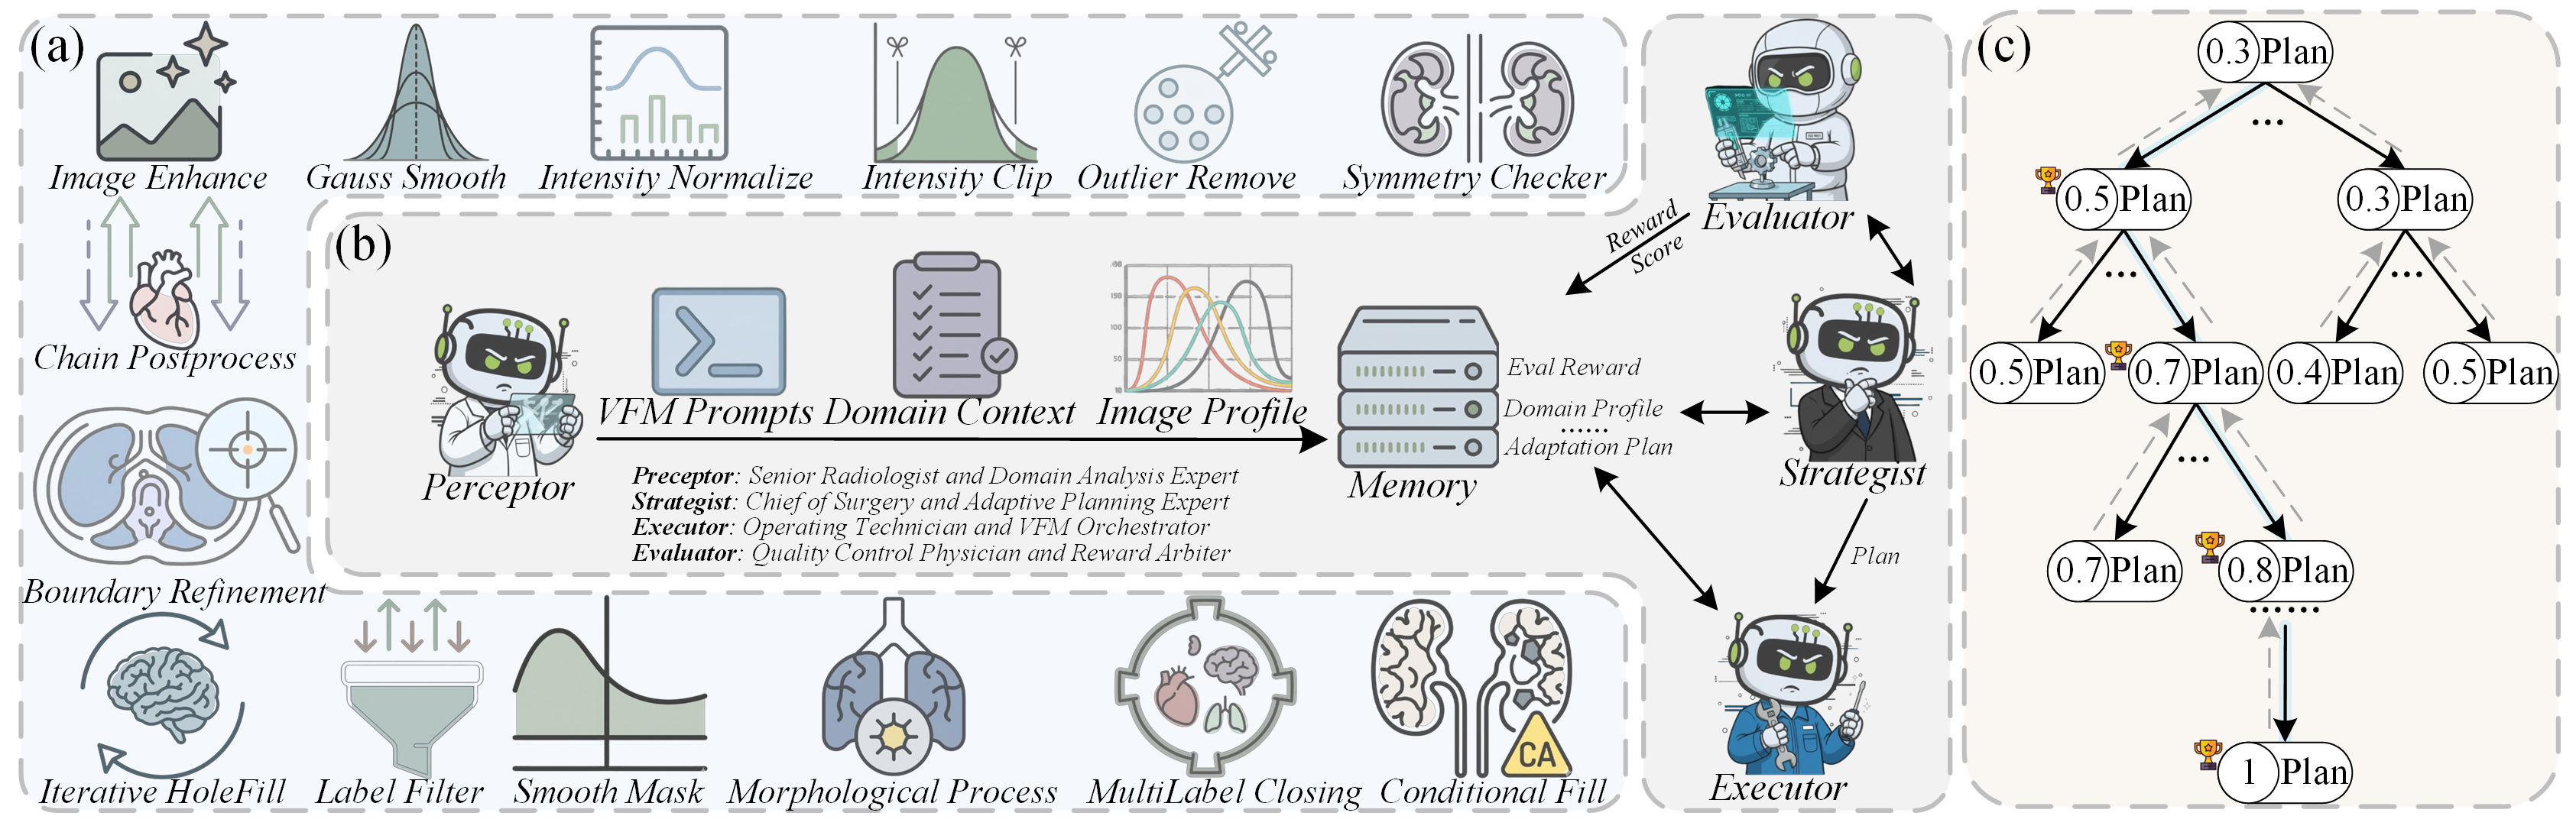
\includegraphics[width=\linewidth]{./Figures/Figure1_WholeFramework.png}
    \vspace{-6mm}
    \caption{Search2Adapt: a multi-agent framework with collaborative tree search for SFUDA. 
    (a) Toolbox of segmentation operators.
    % , including preprocessing, VFM-based generation, and post-processing modules, which together define the action space for pseudo-label refinement.
    (b) Collaborative multi-agent framework.
    % , where Perceptor, Strategist, Executor, and Evaluator interact through a shared memory to form a closed-loop decision-making system for adaptive strategy planning and refinement.
    (c) Example of collaborative tree search.
    % , which performs plan-level exploration over candidate strategies, progressively identifying high-reward refinement plans through structured search and evaluation.
    }
	\label{fig_Overview}
\end{teaserfigure}
%\received{20 February 2007}
%\received[revised]{12 March 2009}
%\received[accepted]{5 June 2009}

%%
%% This command processes the author and affiliation and title
%% information and builds the first part of the formatted document.
\maketitle
\section{Introduction}
Deep learning has achieved remarkable success in medical image analysis when training and deployment share the same data distribution. However, in real-world clinical settings, deep learning models often experience significant performance degradation due to domain shifts arising from differences in imaging modalities, scanner vendors, and acquisition protocols. Such discrepancies between training and deployment distributions are common in multi-center and multi-modality clinical practice, posing a major challenge to reliable clinical deployment. 

Domain adaptation aims to mitigate this issue by leveraging both source and target domain data during model adaptation. In many medical scenarios, however, direct access to source data is strictly limited by privacy regulations and institutional policies. This constraint has led to the emergence of SFUDA, where adaptation is performed using only a pretrained source model and unlabeled target data~\cite{SFUDA_review}. While SFUDA offers an attractive solution for privacy-preserving model deployment, the absence of both source data and target labels makes adaptation inherently challenging.

To address this challenge, various SFUDA methods have been proposed. Most existing approaches follow a static and open-loop adaptation paradigm. They typically rely on predefined pipelines that are uniformly applied across target domains, implicitly assuming that a fixed adaptation strategy is sufficient regardless of domain characteristics. More importantly, these methods lack structured, verifiable feedback mechanisms, as intermediate results generated in early stages are directly used for subsequent optimization without verification and correction. As a result, early errors cannot be effectively detected and propagate throughout the adaptation process, leading to suboptimal performance under domain shifts. These limitations suggest that SFUDA should be viewed as a dynamic decision-making problem that requires adaptive strategy selection.

Recent advances in VLMs have enabled agentic systems capable of perception, reasoning, and tool use, providing a natural foundation for adaptive decision-making. Building on this paradigm, we propose Search2Adapt, which coordinates four specialized agents, Perceptor, Strategist, Executor, and Evaluator, to form a closed-loop system that analyzes target domain characteristics, proposes candidate adaptation plans, executes segmentation operators \cite{monai}, and evaluates intermediate results. To effectively explore the large space of adaptation strategies, we introduce CoTS that performs plan-level exploration to propose adaptation plans, VLM-based reasoning to estimate strategy effectiveness, and employs a diversity-augmented search to balance exploration and exploitation. To enable reliable evaluations, we design a multimodal and anatomy-aware reward that combines geometric feature translation and visual evidence with VLM reasoning based on anatomical priors. In addition, a CoT reflection allows the Strategist to calibrate the Evaluator's evaluation, improving search robustness. Furthermore, a dynamic prior memory accumulates successful adaptation plans across samples, enabling more efficient and stable adaptation. Our contributions are summarized as follows:
\begin{enumerate}[leftmargin=*,noitemsep]
\item We propose Search2Adapt, a multi-agent framework that reformulates SFUDA from executing static adaptation pipelines into a dynamic decision-making problem, thereby transforming open-loop procedures into closed-loop decision processes.
\item We introduce CoTS equipped with a multimodal and anatomy-aware reward, enabling efficient and reliable strategy exploration under SFUDA settings.
\item We develop a CoT-based reflection and a dynamic prior memory that jointly improve search stability and accelerate adaptation through cross-sample knowledge reuse.
\end{enumerate}
\begin{figure}
	\centering
	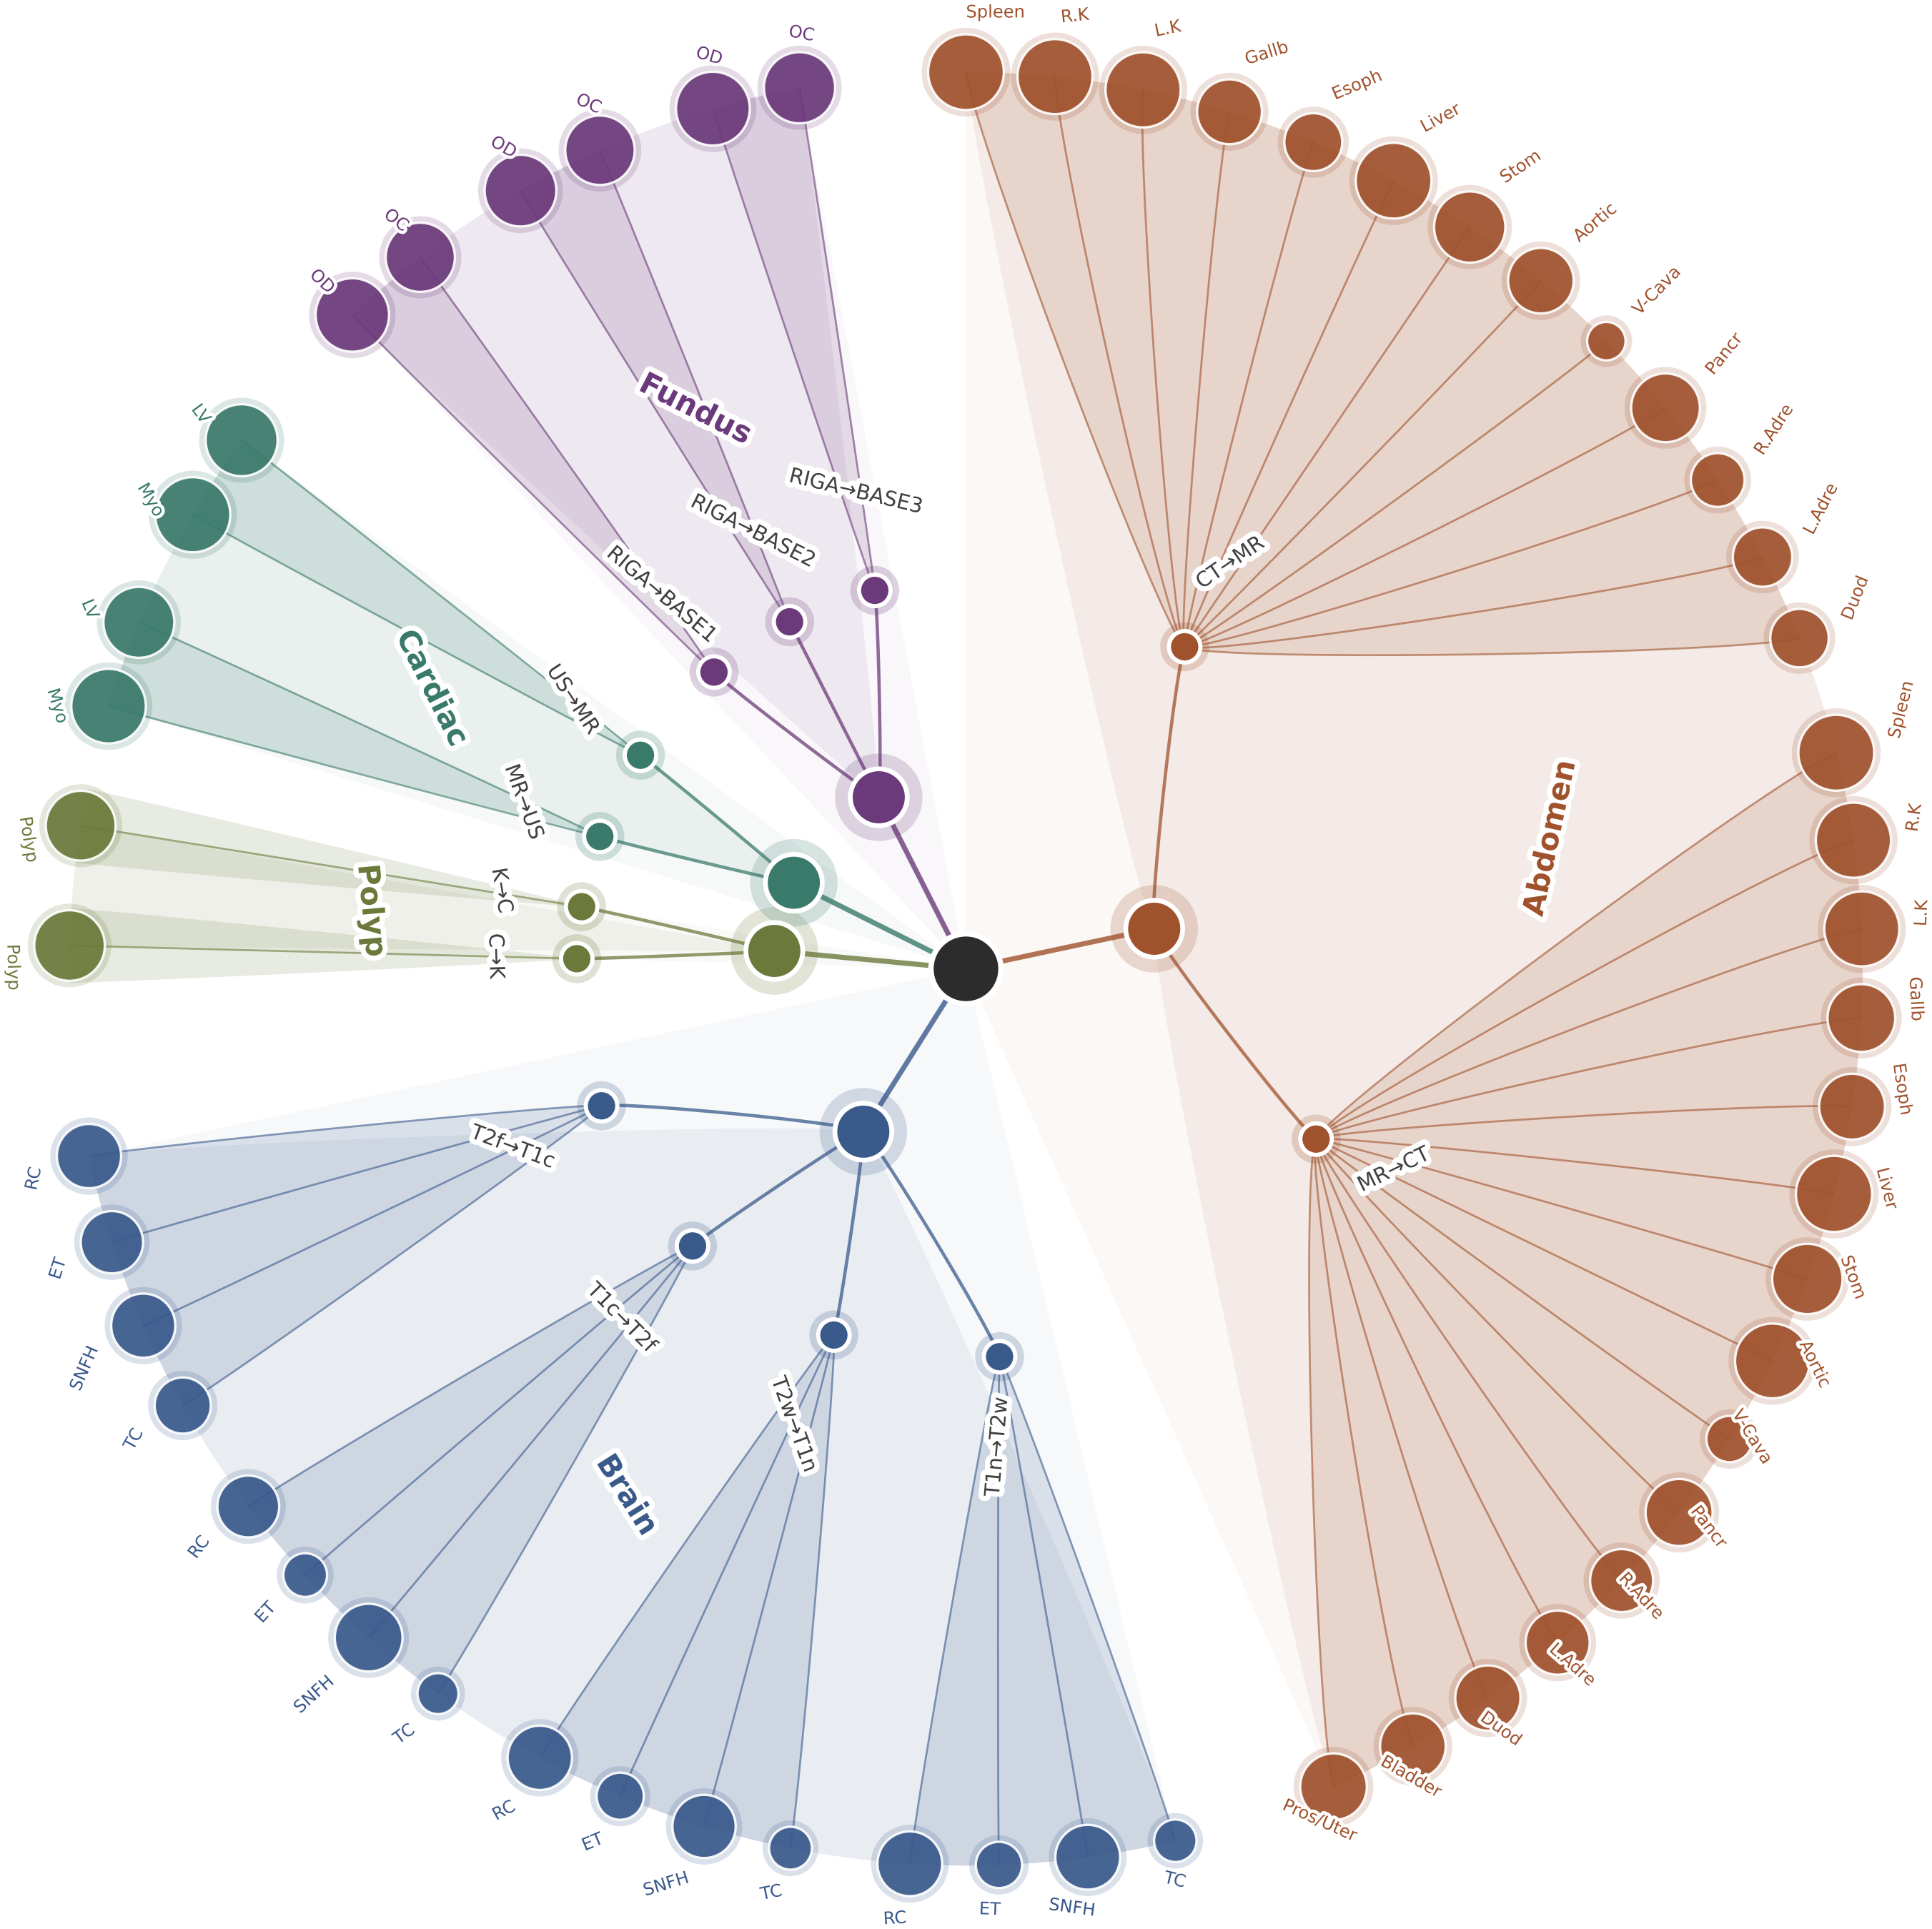
\includegraphics[width=1.05\linewidth]{./Figures/Figure2_TreePlot.png}
    \vspace{-6mm}
    \caption{Generalization of Search2Adapt across 13 domain adaptation directions and 24 anatomy targets. Each branch represents an anatomical target, and each outer node corresponds to an adaptation direction. The size of each outer circle indicates the DICE of adaptation performance. }
	\label{fig_TreePlot}
\vspace{-3mm}
\end{figure}
\section{Related Works}
\subsection{SFUDA for Medical Image Analysis}
SFUDA aims to adapt a pretrained model to an unlabeled target domain without accessing source data~\cite{SFUDA_review}. Existing methods primarily rely on predefined adaptation strategies, including data synthesis, self-training, knowledge distillation, and recent approaches that incorporate VFMs. Data synthesis approaches attempt to approximate the source distribution by generating source-like samples~\cite{Zeng2024ReliableSA}. Self-training methods iteratively refine models using pseudo-labels on target data, often combined with prototype alignment~\cite{protocontra} or uncertainty-aware filtering~\cite{a3dualud}. Knowledge distillation-based approaches adopt teacher-student frameworks to transfer domain-invariant knowledge during adaptation~\cite{IAPC}. More recently, VFM-coupled methods leverage the strong zero-shot segmentation capability of VFMs~\cite{iplc+,SRPL,iplc,prosfda}, typically using pseudo-labels generated by the source model as prompts to guide segmentation.

Despite these advances, most existing approaches still operate under static and open-loop paradigms. Adaptation strategies are predefined and applied uniformly across target domains, without explicitly modeling domain-specific characteristics. Moreover, intermediate results are rarely verified or corrected, causing early-stage errors to propagate throughout the adaptation. This limitation restricts their ability to handle diverse and complex domain shifts.
\begin{figure*}[t]
	\centering
	
\includegraphics[width=\linewidth]{./Figures/Figure3_Detail_Illustration.png}
    \vspace{-6mm}
    \caption{Detailed illustration of the pseudo-label generation process in Search2Adapt.}
	\label{fig_DetailIllustration}
\vspace{-3mm}
\end{figure*}
\subsection{Vision Foundation Models}
VFMs leverage large-scale pretraining to extract transferable visual representations, enabling strong generalization across diverse modalities and domains. Early advancements primarily focused on geometry-aware VFMs, such as SAM~\cite{sam} and its variants (SAM3~\cite{sam3} and MedSAM-3D~\cite{medsam3d}), which excel at capturing shape and boundary information via flexible, prompt-based interaction. While highly effective for structural delineation, these models often lack the domain-specific context required for clinical interpretation. To bridge this gap, semantic-aware VFMs have emerged to integrate high-level knowledge into visual understanding. Models such as BiomedParse~\cite{biomedparse} and SAT~\cite{sat} enable text-guided segmentation and recognition by encoding rich semantic priors of anatomical structures and clinical concepts. Together, these complementary paradigms provide powerful tools for medical image analysis. However, directly deploying such VFMs in clinical edge environments is computationally prohibitive. To overcome these bottlenecks, our framework treats VFMs as frozen, callable knowledge sources within a dynamic search space. Ultimately, we distill their collaborative, zero-shot reasoning knowledge into a lightweight model, achieving a critical balance between high-fidelity adaptation and inference efficiency.

\subsection{Agentic Systems and Search-Based Planning}
Recent advances in VLM have enabled the development of agentic systems capable of perception, reasoning, and tool use \cite{ipo}. In medical image analysis, such systems have been explored to perform complex decision-making processes, including dynamic tool selection and iterative refinement \cite{Li2024AgentHA,zhu2025intelligentagenticcompleximage,coevolvingagent}. By distributing complex problem-solving processes across different agents, these systems can coordinate complementary capabilities and improve robustness.

In parallel, search-based planning algorithms, such as Monte Carlo Tree Search \cite{MCTS_survey}, provide a principled mathematical structure for navigating massive decision spaces. Recent literature has begun to integrate VLM-driven reasoning directly into these search mechanisms \cite{CollaborativeTreeSearch}. Traditionally, tree search relies on an external environment simulator to provide definitive reward signals. In the context of SFUDA, where ground-truth supervision is entirely absent, this dependency is fundamentally limiting. To overcome this, our framework leverages the VLM as an intrinsic, surrogate reward function. By logically assessing intermediate states, the VLM can virtually estimate the anatomical viability of candidate strategies prior. This mechanism provides reliable rewards for guiding exploration and significantly improves search efficiency by pruning unviable paths early, thereby reducing computational overhead.

\section{Method}
\label{sec:method}
Given an unlabeled target dataset $\mathcal{D}_T=\{x_i\}_{i=1}^{N}$, where $x_i\in\mathbb{R}^{H\times W\times D}$ and the goal of SFUDA is to obtain a target adapted model without access to source data. Search2Adapt divides SFUDA into pseudo-label generation and knowledge distillation. Specifically, the pseudo-label generation process is modeled as a sequential decision process, where the state is defined as $s_t=(x_i,\hat{y}_i^{(t)})$. Each action $a_t \in \mathcal{A}$ corresponds to applying a segmentation operator from a defined toolbox $\mathcal{A}$, which serves as the action space containing preprocessing, VFMs, and post-processing operators. A sequence of actions $\pi=(a_1,\dots,a_K)$ defines a refinement strategy, and the objective is to find the optimal strategy $\pi^* = \arg\max_{\pi} R(\pi)$, where $R(\pi)$ evaluates the quality of the resulting pseudo-label.
\subsection{Multi-Agent Collaborative Framework}
To enable adaptive strategy exploration, we delegate the pseudo-label generation process to four specialized agents that interact through a shared memory serving as a global workspace.

\textbf{Perceptor} analyzes target-domain characteristics and produces a domain profile:
$s \rightarrow \text{Profile}$.

\textbf{Strategist} proposes candidate refinement strategies conditioned on the current state and domain profile:
$(s_t,\text{Profile}) \rightarrow \{\pi_1,\pi_2,\dots\}$.

\textbf{Executor} applies the selected strategy deterministically to update the pseudo-label:
$(s_t,\pi) \rightarrow s_{t+1}$.

\textbf{Evaluator} estimates the quality of pseudo-labels and produces a reward signal:
$s_t \rightarrow R \in [0,1]$.

These agents interact in a closed loop through shared memory, enabling iterative refinement, feedback-driven correction, and cross-sample knowledge accumulation.
\subsection{Collaborative Tree Search}
To efficiently explore the strategy space, we introduce CoTS, which performs plan-level search over candidate refinement plan. Each node $v$ in the search tree represents a refinement plan and its corresponding state. During search, nodes are selected according to the Collaborative Action-Value Function (CAVF):
\begin{equation}
\text{CAVF}(v)=V(v)+w\sqrt{\frac{\ln N_{\text{parent}}}{N(v)}}+\lambda D(v), D(v)=\frac{1}{\sqrt{c(\sigma_v)}}
\end{equation}
where $V(v)$ denotes the estimated value, $N(v)$ is the visit count, and $D(v)$ encourages exploration of diverse strategies, and $\sigma_v$ denotes the tool signature of plan $v$, and $c(\sigma_v)$ is the number of previously explored nodes with the same signature. This design discourages repeated exploration of identical tool combinations and promotes strategy diversity.

CoTS follows a two-stage procedure. In the first stage, the Strategist proposes multiple candidate plans, and the Evaluator assesses their effectiveness through CoT reasoning, enabling efficient plan-level exploration. In the second stage, only top-K strategies are executed by the Executor with feasibility monitoring. To further improve robustness, a CoT reflection allows the Strategist to revise evaluation scores when inconsistencies are detected, forming a deliberative interaction between planning and evaluation. The resulting reward is then propagated back to update ancestor nodes.

\subsection{Multimodal and Anatomy-Aware Reward}
Since ground-truth is unavailable in SFUDA, reliable evaluation of pseudo-label quality is critical. Directly applying VLMs to 3D predictions is ineffective due to their limited ability to natively interpret volumetric data.

We address this issue by introducing a multimodal and anatomy-aware reward that fuses visual evidence with programmatic geometric features. To bridge the dimensional gap of volumetric data, we extract a random set of 2D slices, overlay the pseudo-label onto the original images, and compile them into unified visual evidence grids. Concurrently, we extract quantitative geometric features from the predictions, such as the number of connected components, spatial extent, and boundary smoothness, and translate them into structured textual descriptions. By jointly processing the visual evidence grid and the textual geometric profile, the Evaluator agent employs CoT reasoning process to transparently assess the pseudo-label across four critical dimensions: anatomical plausibility ($R_{anat}$), morphological consistency ($R_{morp}$), boundary precision ($R_{bound}$), and false positives ($R_{fp}$). The final reward $R$ is formulated as:
$$R = w_{anat} R_{anat} + w_{morp} R_{morp} + w_{bound} R_{bound} + w_{fp} R_{fp}$$
These weights are integrated into the Evaluator's meta-prompt (Provided in Appendix C) as prioritized guidance, which enables the VLM to dynamically allocate its attention. Evaluator explicitly articulates its diagnostic rationale for each dimension before computing the final reward scores, ensuring the reward assignment is interpretable and grounded in anatomical logic.

\subsection{Shared Memory and Knowledge Distillation}
To improve efficiency and scalability, we maintain a dynamic strategy memory $\mathcal{M}$ that stores successful refinement trajectories discovered during previous searches. Each trajectory is associated with its reward and usage frequency, allowing high-quality strategies to serve as priors for subsequent samples. During CoTS initialization, strategies retrieved from $\mathcal{M}$ are prioritized, significantly accelerating convergence and reducing redundant exploration.

After the search stage, we obtain refined pseudo-labels: $\mathcal{D}_{PL}=\{(x_i,\hat{y}_i^{*})\}$. To enable efficient deployment, we distill the knowledge discovered by the multi-agent search process into a lightweight model. The model parameters are optimized as:
\begin{equation}
\theta_T = \arg\min_{\theta}\sum_{(x,\hat{y})\in\mathcal{D}_{PL}}
\mathcal{L}_{seg}(f(x;\theta),\hat{y})
\end{equation}
where $\mathcal{L}_{seg}$ is a combination of Dice and Cross-Entropy loss. Through this process, the adaptation knowledge is compressed into a lightweight deployable model.
\section{Experiments and Results}
\subsection{Dataset Description}
We conduct extensive experiments across 13 domain adaptation directions and 24 anatomical targets to comprehensively assess the performance of Search2Adapt

\textbf{Abdominal CT/MRI:}
AMOS \cite{amos} comprises multi-center CT and MRI volumes with voxel-wise annotations for 15 abdominal organs, reflecting substantial variations in acquisition protocols and imaging conditions.
\textbf{Brain MRI:}
BraTS-2024 \cite{brats2024}  contains 3D multi-modal MRI scans, including T1n, T1c, T2w, and T2f, with annotations for four tumor-related subregions: enhancing tumor (ET), tumor core (TC), surrounding non-enhancing FLAIR hyperintensity (SNFH), and resection cavity (RC).
\textbf{Cardiac MR/US:}
ACDC \cite{acdc} consists of cardiac MRI scans annotated for the left ventricle (LV), myocardium (MYO), and right ventricle, while CAMUS \cite{CAMUS} provides 2D ultrasound sequences with annotations for LV, MYO, and left atrium. For cross-modality settings (US$\rightarrow$MR and MR$\rightarrow$US), we focus on LV and MYO for consistent evaluation.
\textbf{Polyp Imaging:}
We adopt Kvasir \cite{kvasir} and CVCDB \cite{CVCDB}, two widely used colonoscopy datasets containing pixel-level annotations of polyp regions from endoscopic images and video frames.
\textbf{Fundus Imaging:}
RIGA+ \cite{RIGA+} is a multi-domain retinal dataset for joint optic disc (OD) and optic cup (OC) segmentation, covering five domains. We use the RIGA subset (BinRushed and Magrabia) as source domains and MESSIDOR subset (BASE1, BASE2, BASE3) as target domains.
\begin{algorithm}[t]
\caption{Search2Adapt Framework}
\label{alg:Search2Adapt}
\begin{algorithmic}[1]
\Require Target dataset $\mathcal{D}_T$, source model $f(\cdot;\theta)$, toolbox $\mathcal{A}$, dynamic memory $\mathcal{M}$
\Ensure Target-adapted model $f(\cdot;\theta_T)$

\State $\text{Profile} \leftarrow \textbf{Perceptor}(\mathcal{D}_T)$ \Comment{Extract domain profile}
\State $\mathcal{D}_{PL} \leftarrow \emptyset$ \Comment{Initialize pseudo-label dataset}

\For{each $x_i \in \mathcal{D}_T$}
    \State $\hat{y}_i^{(0)} \leftarrow \text{Generate initial mask for } x_i$ 
    \State $s_0 \leftarrow (x_i, \hat{y}_i^{(0)})$ \Comment{Initialize state}
    
    \State $\Pi_{prior} \leftarrow \textbf{Retrieve}(\mathcal{M}, \text{Profile})$ \Comment{Fetch strategy priors}
    
    \State $\pi^*, \hat{y}_i^*, R^* \leftarrow \textbf{CoTS}(s_0, \text{Profile}, \Pi_{prior}; \mathcal{A})$ %\Comment{Agent-driven search}
    
    \State $\mathcal{M} \leftarrow \textbf{Update}(\mathcal{M}, \pi^*, R^*)$ \Comment{Accumulate knowledge}
    \State $\mathcal{D}_{PL} \leftarrow \mathcal{D}_{PL} \cup \{(x_i, \hat{y}_i^*)\}$
\EndFor

\State $\theta_T \leftarrow \arg\min_{\theta} \sum_{(x,\hat{y})\in \mathcal{D}_{PL}} \mathcal{L}_{seg}(f(x;\theta), \hat{y})$ \Comment{Distillation}

\State \Return $f(\cdot;\theta_T)$
\end{algorithmic}
\end{algorithm}
%\input{algorithm}

\begin{table*}[ht]
\centering
\caption{DICE $\uparrow$ (\%, mean $\pm$ std) of domain adaptation results on abdominal targets. ASD results are provided in the Appendix. } 
\label{tab:AMOS}
\vspace{-2mm}
\resizebox{2\columnwidth}{!}{%
\setlength{\tabcolsep}{2pt}
\begin{tabular}{@{}ccccccccccccccccc@{}}
\toprule
\multicolumn{16}{c}{\textbf{MR$\rightarrow$CT}} \\ \midrule

{ \textbf{Methods}} & { \textbf{Spleen}} & { \textbf{R. K}} & { \textbf{L. K}} & { \textbf{Gallb}} & { \textbf{Esoph}} & { \textbf{Liver}} & { \textbf{Stom}} & { \textbf{Aortic}} & { \textbf{V-Cava}} & { \textbf{Pancr}} & { \textbf{R. Adre}} & { \textbf{L. Adre}} & { \textbf{Duod}} & { \textbf{Bladder}} & { \textbf{Pros/Uter}} & { \textbf{mDICE}} \\ \midrule

{ No Adaptation} & { 65.1$\pm$30.4} & { 71.2$\pm$26.9} & { 63.2$\pm$29.6} & { 27.2$\pm$27.7} & {42.2$\pm$22.1} & {82.2$\pm$9.9} & {46.9$\pm$28.6} & {72.0$\pm$20.3} & {61.7$\pm$23.7} & {55.7$\pm$23.3} & {39.7$\pm$22.8} & {44.7$\pm$24.2} & {38.5$\pm$22.4} & {0.0$\pm$0.0} & {0.0$\pm$0.0} & {47.4$\pm$24.7} \\

{ Supervised} & {97.2$\pm$1.7} & {96.4$\pm$1.7} & {94.7$\pm$11.7} &86.0$\pm$13.6&84.1$\pm$10.0& 97.6$\pm$1.0 & 93.1$\pm$5.1 &95.3$\pm$2.8&90.2$\pm$5.7&83.7$\pm$12.9&77.8$\pm$11.0 &78.9$\pm$11.7 &81.6$\pm$10.9& 83.3$\pm$19.3 &85.5$\pm$7.0 & {88.4$\pm$7.5}\\ \midrule

{ UPL \cite{upl}} & \textcolor{blue}{\textbf{23.9$\pm$2.0}} & {7.7$\pm$0.2} & \textcolor{blue}{\textbf{30.2$\pm$26.9}} & {0.0$\pm$0.0} & {12.5$\pm$12.7} & {23.6$\pm$30.9} & {10.7$\pm$12.2} & {9.3$\pm$10.0} & {0.7$\pm$1.4} & {8.6$\pm$8.3} & {0.0$\pm$0.0} & {0.0$\pm$0.0} & {2.0$\pm$7.2} & {0.0$\pm$0.0} & {0.0$\pm$0.0} & {8.6$\pm$9.4} \\

{ ProtoContra \cite{protocontra}} & {5.6$\pm$6.3} & {11.9$\pm$2.3} & {7.3$\pm$2.6} & \textcolor{blue}{\textbf{4.3$\pm$3.1}} & {37.5$\pm$24.1} &{40.1$\pm$24.8} & {25.1$\pm$21.3} &{38.6$\pm$27.8} & \textcolor{blue}{\textbf{29.2$\pm$18.9}} & {39.1$\pm$20.1} & {0.0$\pm$0.0} & {0.0$\pm$0.0} & {17.6$\pm$16.2} & {0.0$\pm$0.0} & {0.0$\pm$0.0} & {17.1$\pm$15.9} \\

{ IAPC \cite{IAPC}} & {8.7$\pm$4.5} & {4.5$\pm$2.3} & {1.9$\pm$1.4} & {1.3$\pm$1.5} & {4.5$\pm$11.3} & {15.2$\pm$2.1} & {14.3$\pm$5.6} & { 9.7$\pm$5.0} & {4.6$\pm$1.1} & {2.0$\pm$0.6} & {0.0$\pm$0.0} & {0.0$\pm$0.0} & {2.2$\pm$7.4} & \textcolor{blue}{\textbf{19.8$\pm$16.8}} & \textcolor{blue}{\textbf{7.2$\pm$6.8}} & {6.4$\pm$6.1}\\

{ $\diamondsuit$ DFG \cite{DFG}} &{0.7$\pm$0.6} & \textcolor{blue}{\textbf{28.7$\pm$17.4}} & {4.1$\pm$7.2} & {0.0$\pm$0.0} & {35.1$\pm$16.3} & {35.0$\pm$19.2} & {16.6$\pm$16.1} & {13.0$\pm$16.1} & {22.0$\pm$23.3} & {29.7$\pm$18.4} & {0.0$\pm$0.0} & {0.0$\pm$0.0} & {21.2$\pm$12.7} & {0.0$\pm$0.0} & {0.0$\pm$0.0} & {13.7$\pm$13.8}\\

{ $\diamondsuit$ IPLC \cite{iplc}} & {0.0$\pm$0.0} & {0.0$\pm$0.0} & {0.0$\pm$0.0} & {0.0$\pm$0.0} & {0.0$\pm$0.0} & \textcolor{blue}{\textbf{65.4$\pm$11.3}} & {10.5$\pm$7.1} & {6.6$\pm$8.3} & {4.1$\pm$2.7} & {3.8$\pm$3.7} & {0.0$\pm$0.0} & {0.0$\pm$0.0} & {0.0$\pm$0.0} & {0.0$\pm$0.0} & {0.0$\pm$0.0} & { 6.0$\pm$16.7}\\ 

{ $\diamondsuit$ SRPL \cite{SRPL}} & {0.0$\pm$0.0} & {0.0$\pm$0.0} & {0.0$\pm$0.0} & {0.0$\pm$0.0} & \textcolor{blue}{\textbf{41.0$\pm$25.3}} & {47.6$\pm$29.1} & \textcolor{blue}{\textbf{42.2$\pm$26.0}}& \textcolor{blue}{\textbf{66.0$\pm$28.9}} & {26.2$\pm$30.2} & \textcolor{blue}{\textbf{46.6$\pm$23.3}} & {0.0$\pm$0.0} & {0.0$\pm$0.0} & \textcolor{blue}{\textbf{29.4$\pm$17.9}}  & {0.0$\pm$0.0} & {0.0$\pm$0.0} & \textcolor{blue}{\textbf{19.9$\pm$22.9}} \\ \midrule

\textbf{$\diamondsuit$ Ours} & \textcolor{red}{\textbf{96.5$\pm$2.0}} & \textcolor{red}{\textbf{95.3$\pm$4.0}} & \textcolor{red}{\textbf{95.0$\pm$4.7}} & \textcolor{red}{\textbf{82.4$\pm$15.4}} & \textcolor{red}{\textbf{79.1$\pm$12.7}} & \textcolor{red}{\textbf{97.0$\pm$1.8}} & \textcolor{red}{\textbf{86.9$\pm$14.8}} & \textcolor{red}{\textbf{94.6$\pm$2.4}} & \textcolor{red}{\textbf{45.3$\pm$18.8}} & \textcolor{red}{\textbf{81.2$\pm$15.0}} & \textcolor{red}{\textbf{74.2$\pm$13.1}} & \textcolor{red}{\textbf{76.1$\pm$11.1}} & \textcolor{red}{\textbf{78.0$\pm$11.8}} & \textcolor{red}{\textbf{78.8$\pm$24.4}} & \textcolor{red}{\textbf{80.5$\pm$9.9}} & \textcolor{red}{\textbf{82.7$\pm$12.7}}\\

\bottomrule
\end{tabular}%
}

% Lower table: CT->MR with 13 targets
\resizebox{2\columnwidth}{!}{%
\setlength{\tabcolsep}{2pt}
\begin{tabular}{@{}ccccccccccccccc@{}}
\toprule
\multicolumn{14}{c}{\textbf{CT$\rightarrow$MR}} \\ \midrule

{ \textbf{Methods}} & { \textbf{Spleen}} & { \textbf{R. K}} & { \textbf{L. K}} & { \textbf{Gallb}} & { \textbf{Esoph}} & { \textbf{Liver}} & { \textbf{Stom}} & { \textbf{Aortic}} & { \textbf{V-Cava}} & { \textbf{Pancr}} & { \textbf{R. Adre}} & { \textbf{L. Adre}} & { \textbf{Duod}} & { \textbf{mDICE}}\\ \midrule

{ No Adaptation} & { 58.6$\pm$47.0} & { 86.6$\pm$9.2} & { 89.6$\pm$0.7} & {53.1$\pm$28.8} & 58.9$\pm$34.2 & {73.4$\pm$33.0} & 60.0$\pm$19.5 & 61.4$\pm$29.8 & 64.0$\pm$25.1 &65.0$\pm$19.2 & 56.5$\pm$3.3 & 64.7$\pm$10.2 & 44.3$\pm$25.0 &  64.3$\pm$12.5\\

{ Supervised} &97.6$\pm$1.5& 97.1$\pm$0.8&97.1$\pm$0.5&88.1$\pm$10.0 & 73.7$\pm$15.0 &98.0$\pm$1.2 & 90.4$\pm$3.3 & 92.9$\pm$5.2 & 91.7$\pm$2.5 & 86.4$\pm$3.9 &67.7$\pm$9.9 & 71.0$\pm$11.2 & 69.1$\pm$8.7 & 86.2$\pm$10.1\\ \midrule

{ UPL \cite{upl}} & {1.7$\pm$5.3} & {0.8$\pm$1.4} & {2.3$\pm$0.9} & {0.0$\pm$0.0} & {0.0$\pm$0.0} & {12.9$\pm$12.5} & {1.0$\pm$1.1} & {38.4$\pm$19.9} & { 0.0$\pm$0.0} & {12.9$\pm$13.5} & {0.0$\pm$0.0} & {0.0$\pm$0.0} & {0.0$\pm$0.0} & {5.4$\pm$10.0}\\

{ ProtoContra \cite{protocontra}} & {17.8$\pm$16.1} & {4.9$\pm$4.9} & {16.1$\pm$17.8} & {0.0$\pm$0.0} & \textcolor{blue}{\textbf{47.7$\pm$28.0}} & {11.7$\pm$14.4} & {18.7$\pm$14.4} & {6.0$\pm$11.8} & \textcolor{red}{\textbf{38.2$\pm$24.2}} & {30.5$\pm$16.8} & \textcolor{blue}{\textbf{27.3$\pm$22.7}} & {0.0$\pm$0.0} & {0.0$\pm$0.0} & {16.8$\pm$14.5}\\

{ IAPC \cite{IAPC}} & \textcolor{blue}{\textbf{21.9$\pm$3.3}} & {8.9$\pm$3.8} & {19.4$\pm$6.5} & {0.0$\pm$0.0} & {16.1$\pm$6.9} & {13.6$\pm$23.0} & \textcolor{blue}{\textbf{33.8$\pm$3.7}} & {7.8$\pm$1.5} & {2.6$\pm$8.7} & {0.6$\pm$1.0} & {0.0$\pm$0.0} & {0.0$\pm$0.0}  & {0.0$\pm$0.0} & {9.6$\pm$9.9}\\

{ $\diamondsuit$ DFG \cite{DFG}} & {14.0$\pm$12.9} & \textcolor{blue}{\textbf{10.2$\pm$2.7}} & {11.4$\pm$14.7} & {0.0$\pm$0.0} & {36.9$\pm$22.5} & {45.0$\pm$26.9} & {5.9$\pm$10.4} & \textcolor{blue}{\textbf{65.3$\pm$23.3}} & {23.1$\pm$17.7} & {27.3$\pm$22.5} & {0.0$\pm$0.0}  & {0.0$\pm$0.0} & {0.0$\pm$0.0} & {18.4$\pm$19.7} \\

{ $\diamondsuit$ IPLC \cite{iplc}} & {0.0$\pm$0.0} & {0.0$\pm$0.0} & {0.0$\pm$0.0} & {0.0$\pm$0.0} & {2.2$\pm$1.3} & \textcolor{blue}{\textbf{59.6$\pm$13.0}} & {5.0$\pm$2.8} & {10.6$\pm$5.8} & {4.6$\pm$2.9} & {8.4$\pm$6.5} & {0.0$\pm$0.0} & {0.0$\pm$0.0} & {17.6$\pm$2.0} & {7.1$\pm$15.8}\\

{ $\diamondsuit$ SRPL \cite{SRPL}} & {0.0$\pm$0.0} & {0.0$\pm$0.0} & \textcolor{blue}{\textbf{69.8$\pm$24.6}} & {0.0$\pm$0.0} & {0.0$\pm$0.0} & {38.6$\pm$23.9} & {31.1$\pm$26.4} & {54.0$\pm$28.9} & {0.0$\pm$0.0} & \textcolor{blue}{\textbf{42.1$\pm$26.2}} & {0.0$\pm$0.0}& {0.0$\pm$0.0}   & \textcolor{blue}{\textbf{19.7$\pm$17.2}} & \textcolor{blue}{\textbf{19.6$\pm$24.8}}\\ \midrule

{ \textbf{$\diamondsuit$ Ours}} & \textcolor{red}{\textbf{96.2$\pm$1.6}} & \textcolor{red}{\textbf{95.0$\pm$1.2}} & \textcolor{red}{\textbf{95.3$\pm$0.9}} & \textcolor{red}{\textbf{77.4$\pm$20.9}} & \textcolor{red}{\textbf{65.4$\pm$16.6}} & \textcolor{red}{\textbf{96.2$\pm$1.3}} & \textcolor{red}{\textbf{88.5$\pm$4.5}} & \textcolor{red}{\textbf{78.5$\pm$26.0}} & \textcolor{blue}{\textbf{31.7$\pm$20.4}} & \textcolor{red}{\textbf{84.2$\pm$5.8}} & \textcolor{red}{\textbf{58.3$\pm$11.1}} & \textcolor{red}{\textbf{68.0$\pm$11.6}} & \textcolor{red}{\textbf{66.3$\pm$8.4}} & \textcolor{red}{\textbf{77.0$\pm$18.2}}\\ 
\bottomrule
\end{tabular}%
}
\\[2pt]
\footnotesize{~~~~\textit{Note}: A DICE of 0.0 indicates complete prediction failure for the corresponding targets, while the ASD metrics are reported in Appendix A}
\vspace{-5mm}
\end{table*}
\begin{table*}[tbp]
\centering
\caption{DICE $\uparrow$ (\%, mean $\pm$ std) and ASD $\downarrow$ (mm, mean $\pm$ std) of domain adaptation results on brain targets.}
\label{tab:BraTS}
\vspace{-2mm}
\resizebox{2\columnwidth}{!}{%
\renewcommand{\arraystretch}{0.9}  % 减小行距
\setlength{\tabcolsep}{2pt}
\begin{tabular}{@{}c@{\hspace{0.3cm}} cccccccc cccccccc@{}}
\toprule
\multirow{3}{*}{\textbf{Methods}} & \multicolumn{8}{c}{\textbf{T1n$\rightarrow$T2w}} & \multicolumn{8}{c}{\textbf{T2w$\rightarrow$T1n}} \\
\cmidrule(lr){2-9} \cmidrule(lr){10-17}
& \multicolumn{4}{c}{\textbf{DICE}} & \multicolumn{4}{c}{\textbf{ASD}} & \multicolumn{4}{c}{\textbf{DICE}} & \multicolumn{4}{c}{\textbf{ASD}} \\
\cmidrule(lr){2-5} \cmidrule(lr){6-9} \cmidrule(lr){10-13} \cmidrule(lr){14-17}
& \textbf{TC} & \textbf{SNFH} & \textbf{ET} & \textbf{RC} & \textbf{TC} & \textbf{SNFH} & \textbf{ET} & \textbf{RC} & \textbf{TC} & \textbf{SNFH} & \textbf{ET} & \textbf{RC} & \textbf{TC} & \textbf{SNFH} & \textbf{ET} & \textbf{RC} \\ 
\midrule

No Adaptation & 19.7$\pm$29.1 & 7.5$\pm$7.4 & 4.7$\pm$5.6 & 30.0$\pm$24.9 & 40.6$\pm$17.8 &21.2$\pm$8.6 & 40.2$\pm$18.8 & 58.9$\pm$25.7 & 4.6$\pm$4.8 & 13.9$\pm$10.5 & 3.2$\pm$4.9 & 25.9$\pm$38.1 & 48.4$\pm$22.9 & 19.4$\pm$7.6 & 38.1$\pm$15.9 & 57.1$\pm$20.6 \\

Supervised & 61.9$\pm$20.8 & 84.3$\pm$7.3 & 68.0$\pm$14.8 & 86.6$\pm$10.9 & 2.9$\pm$5.1 & 1.3$\pm$0.5 & 1.8$\pm$1.9 & 1.0$\pm$3.0 &62.8$\pm$20.7 &83.6$\pm$6.7& 71.6$\pm$14.9& 83.9$\pm$14.3&2.3$\pm$2.5 & 1.4$\pm$0.6 & 1.8$\pm$2.4 &1.2$\pm$2.9 \\  \midrule

UPL \cite{upl} & \textcolor{red}{\textbf{47.2$\pm$23.4}} & \textcolor{blue}{\textbf{36.9$\pm$22.5}} & \textcolor{red}{\textbf{61.7$\pm$48.6}} & 46.7$\pm$23.5 & 33.6$\pm$22.8 & \textcolor{blue}{\textbf{33.5$\pm$20.8}} & \textcolor{blue}{\textbf{6.8$\pm$6.1}} & \textcolor{blue}{\textbf{29.5$\pm$23.1}} & \textcolor{red}{\textbf{46.5$\pm$34.1}} & 10.7$\pm$12.1 & \textcolor{red}{\textbf{60.3$\pm$48.9}} & \textcolor{blue}{\textbf{38.7$\pm$24.6}} & \textcolor{blue}{\textbf{16.5$\pm$12.8}} & {56.9$\pm$22.1} & \textcolor{blue}{\textbf{23.2$\pm$14.3}} & \textcolor{blue}{\textbf{22.9$\pm$17.0}}\\

ProtoContra \cite{protocontra} & 0.7$\pm$2.3 & 4.9$\pm$12.3 & 6.1$\pm$1.9 & 15.9$\pm$17.8 & \textcolor{blue}{\textbf{19.7$\pm$14.3}} & 52.2$\pm$16.4 & 30.6$\pm$5.6 & {35.0$\pm$16.8} & 0.7$\pm$1.6 & 11.6$\pm$15.1 & 0.4$\pm$3.6 & 0.7$\pm$0.6 & {55.8$\pm$17.5} & 61.4$\pm$22.7 & 36.2$\pm$21.7 & 52.7$\pm$31.6 \\

IAPC \cite{IAPC} & 0.4$\pm$2.3 & {7.2$\pm$10.3} & 2.6$\pm$7.5 & 2.6$\pm$8.2 & 75.7$\pm$42.8 & {72.2$\pm$50.4} & 71.6$\pm$48.3 & 68.7$\pm$44.3 & 0.7$\pm$3.4 & {7.1$\pm$11.1} & 2.2$\pm$6.8 & 3.5$\pm$10.3 & 71.9$\pm$35.7 & 74.3$\pm$52.9 & 66.7$\pm$40.8 & 60.5$\pm$35.2 \\

$\diamondsuit$ DFG \cite{DFG} & {1.3$\pm$1.9} & 3.6$\pm$8.2 & 5.1$\pm$3.8 & 1.6$\pm$7.7 & {50.7$\pm$29.6} & 67.3$\pm$20.5 & {60.7$\pm$23.5} & 53.2$\pm$21.1 & {0.8$\pm$0.6} & 7.6$\pm$14.3 & {4.2$\pm$2.3} & {1.6$\pm$1.2} & 53.9$\pm$22.8 & 63.2$\pm$23.3 & {59.4$\pm$28.2} & {65.7$\pm$22.7} \\

$\diamondsuit$ IPLC \cite{iplc} & 17.8$\pm$3.6 & 20.5$\pm$5.2 & 29.3$\pm$11.2 & \textcolor{blue}{\textbf{52.8$\pm$9.1}} & 27.0$\pm$14.8 & 48.1$\pm$36.3 & 38.1$\pm$16.4 & 53.0$\pm$19.8 & 25.7$\pm$16.8 & \textcolor{blue}{\textbf{30.0$\pm$12.3}} & 39.7$\pm$32.9 & 16.2$\pm$17.4 & 47.2$\pm$46.1 & 36.7$\pm$23.2 & 36.3$\pm$17.6 & 45.4$\pm$17.7 \\ 

$\diamondsuit$ SRPL \cite{SRPL}  & 0.0$\pm$0.0 & 13.3$\pm$13.3 & 10.7$\pm$12.2 & 3.3$\pm$3.3 & 63.2$\pm$33.2 & 35.2$\pm$24.1 & 73.3$\pm$34.5 & 55.4$\pm$22.1 & 8.4$\pm$13.5 & 9.2$\pm$7.7 & 9.9$\pm$10.7 & 2.5$\pm$2.3 & 70.8$\pm$30.0 & \textcolor{blue}{\textbf{25.9$\pm$9.8}} & 50.7$\pm$24.4 & 51.3$\pm$13.8\\ \midrule

\textbf{$\diamondsuit$ Ours} & \textcolor{blue}{\textbf{38.7$\pm$23.5}} & \textcolor{red}{\textbf{77.3$\pm$11.3}} & \textcolor{blue}{\textbf{45.3$\pm$23.6}} & \textcolor{red}{\textbf{77.2$\pm$18.7}}& \textcolor{red}{\textbf{6.7$\pm$9.7}} & \textcolor{red}{\textbf{1.8$\pm$1.2}}& \textcolor{red}{\textbf{6.0$\pm$10.0}} & \textcolor{red}{\textbf{2.5$\pm$5.0}} & \textcolor{blue}{\textbf{39.4$\pm$26.0}} & \textcolor{red}{\textbf{74.7$\pm$14.3}} & \textcolor{blue}{\textbf{46.8$\pm$22.2}} & \textcolor{red}{\textbf{76.5$\pm$21.1}} & \textcolor{red}{\textbf{5.4$\pm$6.5}} & \textcolor{red}{\textbf{2.1$\pm$2.0}} & \textcolor{red}{\textbf{4.5$\pm$6.7}} & \textcolor{red}{\textbf{2.6$\pm$5.7}} \\ 


\midrule
\midrule

\multirow{3}{*}{\textbf{Methods}} & \multicolumn{8}{c}{\textbf{T1c$\rightarrow$T2f}} & \multicolumn{8}{c}{\textbf{T2f$\rightarrow$T1c}} \\
\cmidrule(lr){2-9} \cmidrule(lr){10-17}
& \multicolumn{4}{c}{\textbf{DICE}} & \multicolumn{4}{c}{\textbf{ASD}} & \multicolumn{4}{c}{\textbf{DICE}} & \multicolumn{4}{c}{\textbf{ASD}} \\
\cmidrule(lr){2-5} \cmidrule(lr){6-9} \cmidrule(lr){10-13} \cmidrule(lr){14-17}
& \textbf{TC} & \textbf{SNFH} & \textbf{ET} & \textbf{RC} & \textbf{TC} & \textbf{SNFH} & \textbf{ET} & \textbf{RC} & \textbf{TC} & \textbf{SNFH} & \textbf{ET} & \textbf{RC} & \textbf{TC} & \textbf{SNFH} & \textbf{ET} & \textbf{RC} \\ 
\midrule

No Adaptation & 4.8$\pm$5.7 & 1.3$\pm$1.4 & 14.2$\pm$15.1 & 49.3$\pm$33.5 & 39.9$\pm$30.7 & 22.7$\pm$7.9 &33.8$\pm$19.2 & 26.3$\pm$26.9 & 18.8$\pm$19.9 & 2.1$\pm$3.6 & 42.7$\pm$25.7 & 54.0$\pm$33.1 & 10.8$\pm$13.9 & 23.8$\pm$18.4 & 6.4$\pm$7.7 & 11.6$\pm$19.6 \\

Supervised & 63.1$\pm$20.2 & 90.3$\pm$5.6 &66.6$\pm$15.2 &83.7$\pm$11.4&2.5$\pm$2.5& 0.97$\pm$0.4& 2.2$\pm$2.7 &1.0$\pm$0.7& 82.4$\pm$15.3 & 83.6$\pm$6.9& 84.8$\pm$12.5&85.3$\pm$14.1 & 1.4$\pm$5.0& 1.4$\pm$0.5&0.8$\pm$0.9 &1.0$\pm$1.5 \\ \midrule

UPL \cite{upl} &\textcolor{blue}{\textbf{25.0$\pm$22.0}} &46.6$\pm$19.4 &22.6$\pm$16.3 &\textcolor{blue}{\textbf{55.9$\pm$30.2}}& \textcolor{blue}{\textbf{32.9$\pm$22.5}} & {26.1$\pm$23.8} &36.9$\pm$24.0 &29.7$\pm$26.6 & \textcolor{blue}{\textbf{43.4$\pm$27.1}} & 15.6$\pm$15.6 & \textcolor{blue}{\textbf{44.6$\pm$26.1}} & \textcolor{blue}{\textbf{53.7$\pm$29.1}} & \textcolor{blue}{\textbf{28.6$\pm$25.5}} & 46.2$\pm$22.2 & \textcolor{blue}{\textbf{27.6$\pm$23.9}} & \textcolor{blue}{\textbf{29.7$\pm$26.8}} \\

ProtoContra \cite{protocontra} & {0.1$\pm$1.3} & \textcolor{blue}{\textbf{58.4$\pm$27.5}} & 12.1$\pm$5.6 & 14.4$\pm$25.5 & {51.5$\pm$27.6}& \textcolor{blue}{\textbf{18.0$\pm$19.8}} & 38.0$\pm$21.4 & \textcolor{blue}{\textbf{25.8$\pm$20.5}} & 2.6$\pm$9.8 & 15.5$\pm$17.9 & 11.6$\pm$21.1 & 13.0$\pm$26.0 &{53.1$\pm$24.4} & 50.0$\pm$24.8 & 47.8$\pm$25.4 & 34.1$\pm$27.4 \\

IAPC \cite{IAPC} & 1.0$\pm$4.6 & 6.9$\pm$10.5 & 2.3$\pm$7.5 & 29.4$\pm$9.2 & 69.1$\pm$35.7 & 68.8$\pm$48.2 & 59.7$\pm$35.4 & 62.1$\pm$37.6 & 13.2$\pm$5.0 & 6.7$\pm$11.1 & 4.2$\pm$8.9 & 3.8$\pm$10.0 & 65.6$\pm$32.6 & 77.5$\pm$58.3 & 64.9$\pm$43.3 & 80.6$\pm$60.1 \\

$\diamondsuit$ DFG \cite{DFG} & {0.2$\pm$3.2} & 9.2$\pm$12.5 & {6.6$\pm$3.1} & {4.3$\pm$12.9} & {65.0$\pm$20.2} & 49.1$\pm$22.0 & {58.6$\pm$24.5} & {50.7$\pm$27.1} & {1.3$\pm$1.8} & {3.6$\pm$8.2} & {5.1$\pm$3.1} & {1.6$\pm$7.7} & {50.7$\pm$29.6} & 67.3$\pm$20.5 & {60.7$\pm$23.5} & 53.2$\pm$21.0 \\

$\diamondsuit$ IPLC \cite{iplc} & 17.6$\pm$8.3 & 42.8$\pm$15.6 & \textcolor{red}{\textbf{39.9$\pm$6.1}} & 28.7$\pm$13.2 & 55.1$\pm$33.4 & 48.2$\pm$42.9 & 34.6$\pm$33.9 & 27.2$\pm$16.1 & 29.6$\pm$24.4 & \textcolor{blue}{\textbf{39.9$\pm$18.1}} & 13.7$\pm$7.4 & 44.8$\pm$18.6 & 43.9$\pm$28.1 & \textcolor{blue}{\textbf{19.2$\pm$8.4}} & 59.4$\pm$47.0 & 33.0$\pm$19.9 \\

$\diamondsuit$ SRPL \cite{SRPL} & 15.9$\pm$18.2 & 3.8$\pm$4.1 & 23.3$\pm$18.6 & 5.5$\pm$8.2 & 40.2$\pm$35.1 & 30.6$\pm$12.5 & \textcolor{blue}{\textbf{34.5$\pm$30.9}} & 30.2$\pm$24.3 & 24.1$\pm$20.7 & 7.4$\pm$7.0 & 22.3$\pm$20.2 & 6.5$\pm$8.0 & 36.4$\pm$46.0 & 27.7$\pm$12.3 & 45.0$\pm$37.5 & 39.0$\pm$21.5 \\ \midrule

\textbf{$\diamondsuit$ Ours} & \textcolor{red}{\textbf{36.1$\pm$25.6}} & \textcolor{red}{\textbf{82.4$\pm$10.5}} & \textcolor{blue}{\textbf{40.8$\pm$24.0}} & \textcolor{red}{\textbf{72.1$\pm$24.3}}   &\textcolor{red}{\textbf{8.4$\pm$8.8}} & \textcolor{red}{\textbf{1.4$\pm$0.7}} & \textcolor{red}{\textbf{5.2$\pm$6.6}} & \textcolor{red}{\textbf{2.4$\pm$5.4}} & \textcolor{red}{\textbf{62.4$\pm$25.7}} & \textcolor{red}{\textbf{76.2$\pm$11.7}} & \textcolor{red}{\textbf{73.0$\pm$20.1}} & \textcolor{red}{\textbf{76.4$\pm$20.9}} & \textcolor{red}{\textbf{3.9$\pm$8.4}} & \textcolor{red}{\textbf{2.0$\pm$1.4}} & \textcolor{red}{\textbf{1.7$\pm$2.5}} & \textcolor{red}{\textbf{2.6$\pm$6.4}} \\ 

\bottomrule
\end{tabular}%
}
\vspace{-3mm}
\end{table*}
\subsection{Implementation and Experiments Details}
All experiments were implemented using PyTorch and conducted on an NVIDIA RTX 4090 GPU. We utilized nnUNet as our source model, which employs a ResNet-based architecture pre-trained for 300 epochs. Building upon this, a lightweight student model initialized from the source model was adapted to the target domain via knowledge distillation for 300 epochs. To drive the Search2Adapt, we employed the Qwen3.5-0.8B-GGUF-Q4-K-XL \cite{qwen3.5}, accelerated by Unsloth \cite{unsloth}, and applied unified meta-prompts across all adaptation directions. During the search phase, the CAVF exploration weight $w$ and the diversity coefficient $\lambda$ were set to $\sqrt{2}$ and 0.1, respectively. Additionally, both the number of candidate plan variants and the top-$K$ execution budget were fixed at 4. For the experimental setup, all target images were randomly divided into training and test sets in an 8:2 ratio. Crucially, the pseudo-label generation and knowledge distillation processes were strictly confined to the training split. Finally, we evaluated the adaptation performance using the Dice similarity coefficient (DICE) and Average Surface Distance (ASD), reporting the results as mean $\pm$ std across all samples. Further implementation details, including the specific meta-prompts and the Evaluator's toolbox, are provided in the Appendix to ensure full reproducibility.
\begin{figure*}[t]
	\centering
	
\includegraphics[width=\linewidth]{./Figures/Figure4_Example_Result.png}
    \vspace{-6mm}
    \caption{Qualitative results of Search2Adapt demonstrate strong generalization across diverse and challenging domain adaptation directions after adaptation. Specifically, the first and second rows show adaptation to abdominal targets, while the third row shows adaptation to cardiac, polyp, and brain targets.}
	\label{fig_ExampleResult}
\vspace{-3mm}
\end{figure*}
\subsection{Comparison with SOTA Methods}
We compare Search2Adapt with six SOTA SFUDA methods, covering both medical-purpose approaches (UPL \cite{upl}, ProtoContra \cite{protocontra}, DFG \cite{DFG}, IPLC \cite{iplc}, SRPL \cite{SRPL}) and general-purpose approaches (IAPC \cite{IAPC}). Notably, our evaluation aligns with the emerging paradigm of VFM-coupled SFUDA, in which DFG and IPLC use MedSAM, while SRPL is built on SAM. The remaining methods are traditional SFUDA methods that do not use VFM. In our experiments, \textbf{No Adaptation} denotes the source model tested directly on the target domain without adaptation, while \textbf{Supervised} denotes training and testing on the target domain with full supervision.
\begin{table*}[t]
\centering
\caption{DICE $\uparrow$ (\%, mean $\pm$ std) and ASD $\downarrow$ (mm, mean $\pm$ std) of domain adaptation results on cardiac and polyp targets.}
\label{tab:Cardiac_Polyp}
\vspace{-2mm}
\resizebox{\textwidth}{!}{%
\renewcommand{\arraystretch}{0.75}
\begin{tabular}{@{}c@{\hspace{0.25cm}} cccc cccc @{\hspace{0.4cm}} cc cc@{}}
\toprule
% 表头第一层
\multirow{3}{*}{\textbf{Methods}} & \multicolumn{8}{c}{\textbf{Cardiac}} & \multicolumn{4}{c}{\textbf{Polyp}} \\
\cmidrule(lr){2-9} \cmidrule(lr){10-13}
% 表头第二层
& \multicolumn{4}{c}{\textbf{MR$\rightarrow$US}} & \multicolumn{4}{c}{\textbf{US$\rightarrow$MR}} & \multicolumn{2}{c}{\textbf{Kvasir$\rightarrow$CVCDB}} & \multicolumn{2}{c}{\textbf{CVCDB$\rightarrow$Kvasir}} \\
\cmidrule(lr){2-5} \cmidrule(lr){6-9} \cmidrule(lr){10-11} \cmidrule(lr){12-13}
% 表头第三层
& \multicolumn{2}{c}{\textbf{DICE}} & \multicolumn{2}{c}{\textbf{ASD}} & \multicolumn{2}{c}{\textbf{DICE}} & \multicolumn{2}{c}{\textbf{ASD}} & \textbf{DICE} & \textbf{ASD} & \textbf{DICE} & \textbf{ASD} \\
\cmidrule(lr){2-3} \cmidrule(lr){4-5} \cmidrule(lr){6-7} \cmidrule(lr){8-9}
% 表头第四层
& \textbf{LV} & \textbf{MYO} & \textbf{LV} & \textbf{MYO} & \textbf{LV} & \textbf{MYO} & \textbf{LV} & \textbf{MYO} & & & & \\ 
\midrule
No Adaptation & 1.7$\pm$0.7 & 3.1$\pm$0.3 & 56.2$\pm$37.2 & 66.9$\pm$42.3 & 3.2$\pm$0.6 & 1.8$\pm$0.3 & 60.5$\pm$34.9 & 56.8$\pm$27.5 & 65.1$\pm$21.5 & 5.8$\pm$11.1 & 60.2$\pm$27.0 & 23.7$\pm$20.4 \\
Supervised & 94.4$\pm$2.7 & 88.1$\pm$4.6 & 3.2$\pm$1.6 & 4.1$\pm$1.3 & 95.8$\pm$3.8 & 91.2$\pm$2.1 & 0.3$\pm$0.1 & 0.3$\pm$0.1 & 99.8$\pm$0.1 & 0.36$\pm$0.1 & 97.4$\pm$1.3 & 0.9$\pm$1.1 \\ 
\midrule
UPL \cite{upl} & 2.8$\pm$0.1 & 0.0$\pm$0.0 & 90.5$\pm$3.2 & N/A & 0.5$\pm$0.4 & 2.9$\pm$2.1 & 88.9$\pm$9.6 & 85.6$\pm$11.6 & 67.1$\pm$14.6 & \textcolor{blue}{\textbf{2.2$\pm$0.9}} & 60.2$\pm$31.3 & 11.4$\pm$17.2 \\
ProtoContra \cite{protocontra} & 1.2$\pm$1.2 & \textcolor{blue}{\textbf{17.0$\pm$7.2}} & 54.9$\pm$14.2 & 56.4$\pm$13.9 & 5.2$\pm$5.8 & 4.9$\pm$3.2 & 72.9$\pm$12.4 & 74.8$\pm$10.5 & \textcolor{blue}{\textbf{78.0$\pm$12.1}} & \textcolor{red}{\textbf{0.9$\pm$0.6}} & \textcolor{blue}{\textbf{68.9$\pm$26.4}} & \textcolor{red}{\textbf{9.5$\pm$15.0}} \\
IAPC \cite{IAPC} & \textcolor{blue}{\textbf{18.4$\pm$14.5}} & 3.1$\pm$7.5 & 51.3$\pm$29.6 & 97.9$\pm$45.3 & \textcolor{blue}{\textbf{25.8$\pm$15.2}} & 5.6$\pm$0.8 & {34.1$\pm$13.9} & 42.6$\pm$12.7 & 73.3$\pm$29.6 & 4.4$\pm$7.9 & 61.2$\pm$26.3 & 13.7$\pm$13.2 \\
$\diamondsuit$DFG \cite{DFG} & 4.6$\pm$4.1 & 4.5$\pm$3.7 & 51.6$\pm$12.9 & 63.1$\pm$14.3 & 2.3$\pm$1.7 & 6.9$\pm$4.4 & 69.3$\pm$16.7 & 66.5$\pm$18.3 & 19.1$\pm$14.7 & 97.5$\pm$17.6 & 26.8$\pm$18.1 & 87.5$\pm$19.5 \\
$\diamondsuit$IPLC \cite{iplc} & 1.7$\pm$2.0 & 5.8$\pm$2.5 & \textcolor{blue}{\textbf{50.5$\pm$18.1}} & \textcolor{blue}{\textbf{48.3$\pm$18.9}} & 2.9$\pm$3.6 & \textcolor{blue}{\textbf{11.5$\pm$8.9}} & 48.4$\pm$11.2 & \textcolor{blue}{\textbf{26.1$\pm$10.5}} & 34.8$\pm$11.7 & 34.7$\pm$22.9 & 45.3$\pm$21.2 & 19.2$\pm$8.4 \\
$\diamondsuit$SRPL \cite{SRPL} & 0.7$\pm$1.1 & 0.9$\pm$1.2 & 83.1$\pm$31.0 & 79.8$\pm$19.2 & 8.5$\pm$9.3 & 9.1$\pm$9.3 & \textcolor{blue}{\textbf{30.1$\pm$15.3}} & 45.9$\pm$22.0 & 33.0$\pm$22.7 & 31.4$\pm$19.6 & 44.9$\pm$26.0 & 18.9$\pm$16.9 \\ 
\midrule
$\diamondsuit$\textbf{Ours} & \textcolor{red}{\textbf{87.9$\pm$4.7}} & \textcolor{red}{\textbf{94.2$\pm$2.8}} & \textcolor{red}{\textbf{3.0$\pm$0.8}} & \textcolor{red}{\textbf{2.2$\pm$0.4}} & \textcolor{red}{\textbf{89.7$\pm$3.6}} & \textcolor{red}{\textbf{95.2$\pm$3.8}} & \textcolor{red}{\textbf{0.3$\pm$0.1}} & \textcolor{red}{\textbf{0.2$\pm$0.1}}& \textcolor{red}{\textbf{86.0$\pm$18.1}} & {7.1$\pm$12.1} & \textcolor{red}{\textbf{87.4$\pm$16.3}} & \textcolor{blue}{\textbf{10.6$\pm$15.9}} \\ 
\bottomrule
\end{tabular}%
}
\vspace{-3mm}
\end{table*}

\textbf{Results on Abdominal Targets}
Table~\ref{tab:AMOS} summarizes the quantitative results on abdominal targets in MR$\rightarrow$CT and CT$\rightarrow$MR. In MR$\rightarrow$CT, Search2Adapt achieves a mean DICE of 82.7\%, substantially outperforming all existing SFUDA methods and closely approaching \textbf{Supervised} (88.4\%). Notably, our method consistently delivers high DICE across both large and small organs, including the spleen (96.5\%), liver (97.0\%), and pancreas (81.2\%), whereas most competing methods suffer from widespread prediction failures. Similar trends are observed in CT$\rightarrow$MR. Search2Adapt achieves a mean DICE of 77.0\%, significantly exceeding other SFUDA methods and narrowing the gap to \textbf{Supervised} (86.2\%). Despite these overall improvements, we observe suboptimal performance on the vena cava (45.3\% in MR$\rightarrow$CT and 31.7\% in CT$\rightarrow$MR). This local degradation is attributable to certain refinement operators in our toolbox, such as Gaussian smoothing, which can inadvertently over-smooth continuous tubular structures during the adaptation process. Nevertheless, these results highlight the overall effectiveness of Search2Adapt in improving adaptation performance and validating its robustness across the vast majority of the 15 distinct anatomical targets.

\textbf{Results on Brain Targets}
Table~\ref{tab:BraTS} reports the performance of Search2Adapt on brain targets. In T1n$\rightarrow$T2w, Search2Adapt achieves a strong DICE of 77.3\% on SNFH and 77.2\% on RC, substantially outperforming \textbf{No Adaptation} and existing SFUDA methods. While improvements in smaller, more ambiguous regions such as TC and ET are more moderate, Search2Adapt maintains consistently low ASDs (1.8\,mm on SNFH and 2.5\,mm on RC), indicating reliable boundary precision under severe domain shifts. Similar trends are observed in T2w$\rightarrow$T1n, where Search2Adapt again delivers high DICE on SNFH (74.7\%) and RC (76.5\%) along with the lowest ASD.

The advantage of Search2Adapt becomes more pronounced in post-contrast adaptation scenarios. In T1c$\rightarrow$T2f, our method achieves a DICE of 82.4\% on SNFH and 72.1\% on RC, closely approaching \textbf{Supervised}, while reducing the ASD of SNFH to 1.4\,mm. Likewise, in T2f$\rightarrow$T1c, Search2Adapt attains consistently high DICE across all tumor subregions (76.2\% on SNFH and 76.4\% on RC) with superior boundary accuracy. Compared with prior SFUDA methods, which often favor specific subregions or exhibit large ASD, Search2Adapt provides more balanced improvements across both DICE and ASD.

\begin{figure*}
	\centering
	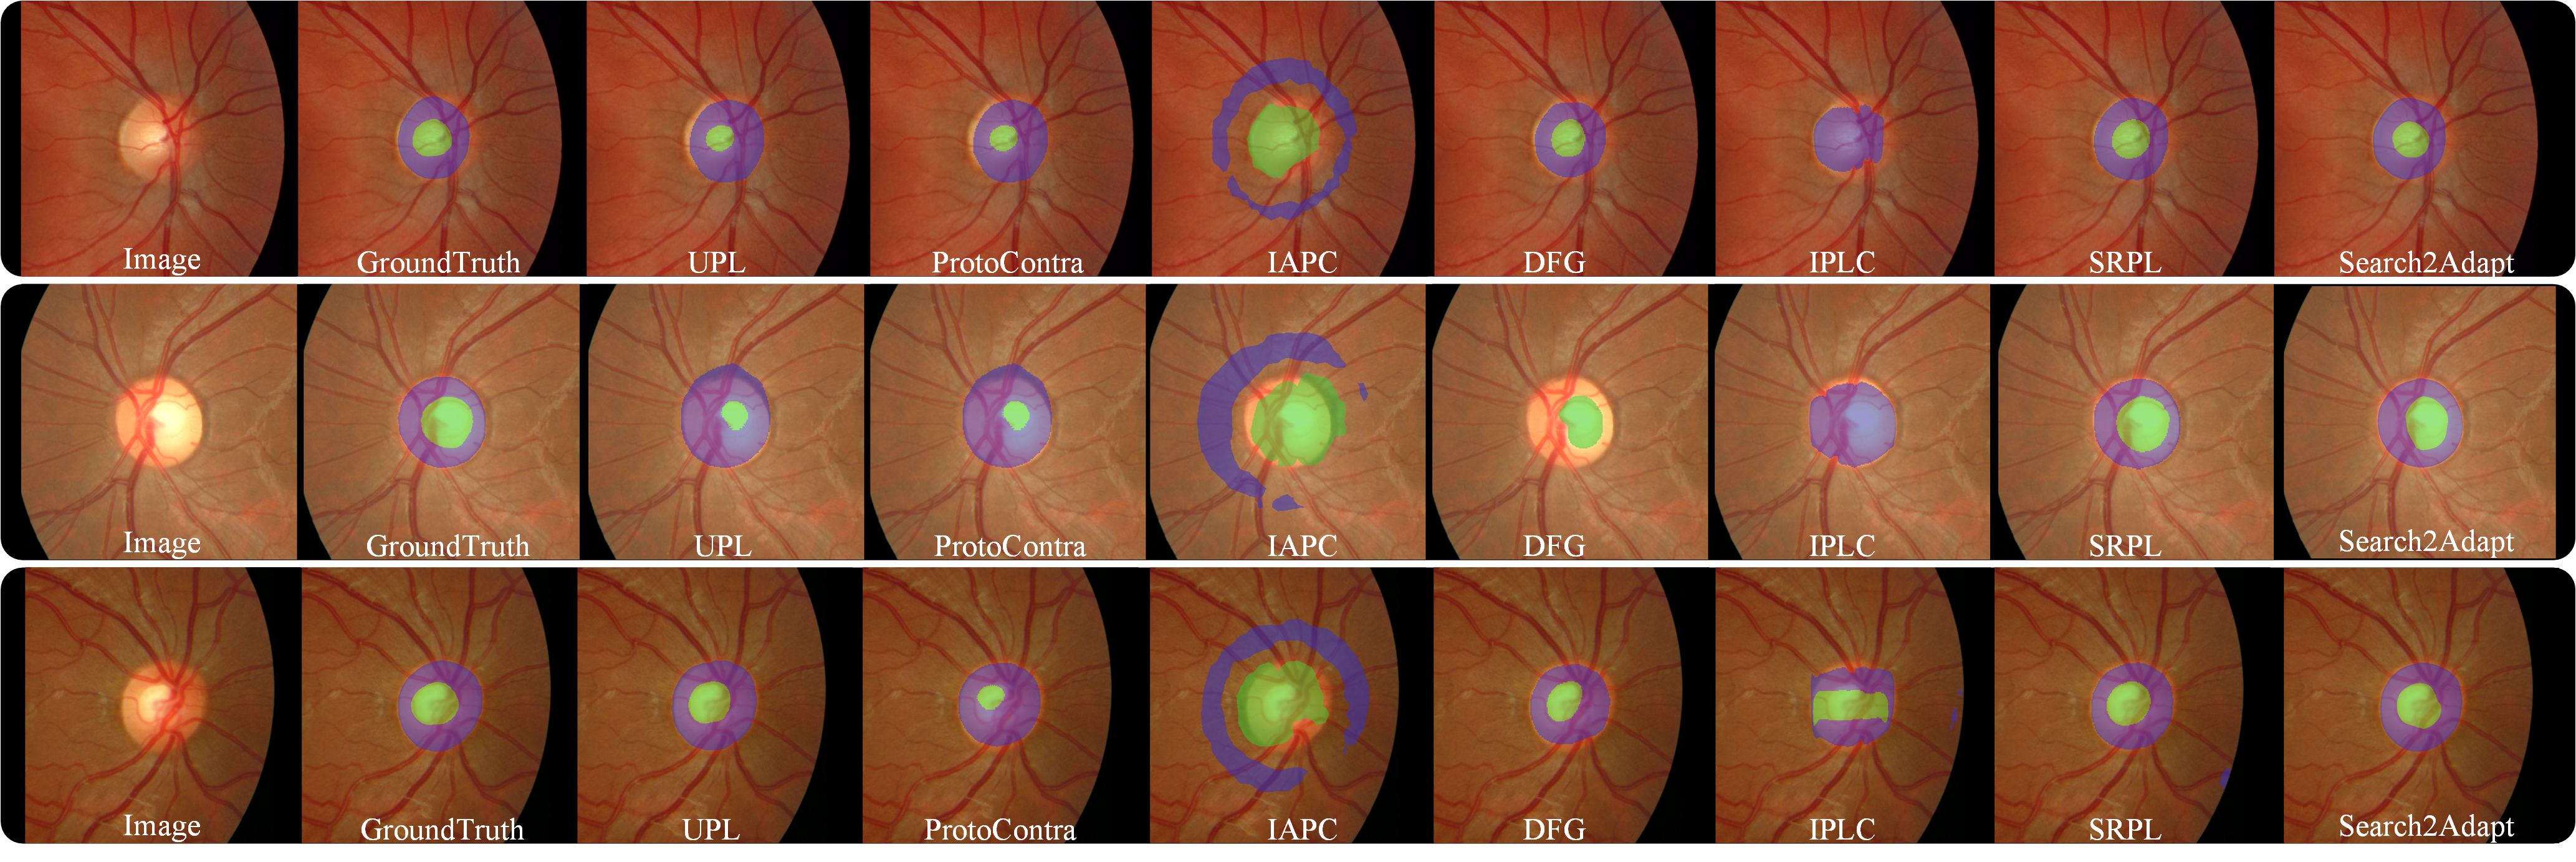
\includegraphics[width=\linewidth]{./Figures/Figure5_Fundus_Result.png}
    \vspace{-6mm}
    \caption{Qualitative results from source domain RIGA to targets BASE1, BASE2, and BASE3 (top to bottom).}
	\label{fig_Fundus}
\vspace{-3mm}
\end{figure*}
\begin{table}[tbp]
\centering
\caption{DICE and ASD of domain adaptation results on fundus targets. The source domain is fixed to RIGA, while BASE1, BASE2, and BASE3 are target domains.}
\label{tab:Fundus}
\resizebox{\columnwidth}{!}{%
\setlength{\tabcolsep}{2pt}          % ← 新增：收窄列间距（默认 6pt）
\footnotesize                         % ← 新增：字号降一级，整体更紧凑
\begin{tabular}{@{}c@{\hspace{0.15cm}} cccccc cccccc@{}}  % ← hspace 从 0.3cm → 0.15cm
\toprule
\multirow{3}{*}{\textbf{Methods}} & \multicolumn{6}{c}{\textbf{DICE}} & \multicolumn{6}{c}{\textbf{ASD}} \\
\cmidrule(lr){2-7} \cmidrule(lr){8-13}
& \multicolumn{2}{c}{\textbf{BASE1}} & \multicolumn{2}{c}{\textbf{BASE2}} & \multicolumn{2}{c}{\textbf{BASE3}} & \multicolumn{2}{c}{\textbf{BASE1}} & \multicolumn{2}{c}{\textbf{BASE2}} & \multicolumn{2}{c}{\textbf{BASE3}} \\
\cmidrule(lr){2-3} \cmidrule(lr){4-5} \cmidrule(lr){6-7} \cmidrule(lr){8-9} \cmidrule(lr){10-11} \cmidrule(lr){12-13}
& \textbf{OD} & \textbf{OC} & \textbf{OD} & \textbf{OC} & \textbf{OD} & \textbf{OC} & \textbf{OD} & \textbf{OC} & \textbf{OD} & \textbf{OC} & \textbf{OD} & \textbf{OC} \\ 
\midrule
No Adaptation & {83.5$\pm$3.4} & {72.6$\pm$15.7} & {79.5$\pm$4.2} & {73.7$\pm$12.4} & {82.8$\pm$3.5} & {78.2$\pm$9.1} & {7.2$\pm$2.3} & {13.9$\pm$8.8} & {5.8$\pm$3.3} & {9.2$\pm$7.8} & {10.7$\pm$8.8} & {10.1$\pm$4.6} \\
Supervised & {94.5$\pm$1.5} & {91.6$\pm$4.1} & {93.7$\pm$2.4} & {92.1$\pm$3.8} & {94.2$\pm$2.0} & {92.8$\pm$3.6} & {3.6$\pm$3.8} & {4.7$\pm$1.8} & {3.4$\pm$1.4} & {4.4$\pm$1.9} & {3.2$\pm$1.3} & {4.2$\pm$1.6} \\ 
\midrule
UPL \cite{upl} & 87.3$\pm$4.7 &{81.7$\pm$11.9} & {80.4$\pm$10.1} & {80.4$\pm$9.3} & {88.4$\pm$5.8} & {84.7$\pm$6.7} & {7.4$\pm$3.1} & {9.8$\pm$8.6} & {48.1$\pm$42.5} & {10.4$\pm$5.0} & {8.4$\pm$11.2} & 10.6$\pm$11.4 \\
ProtoContra \cite{protocontra} & {75.4$\pm$11.1} & {62.4$\pm$15.6} & {64.7$\pm$12.1} & {47.1$\pm$15.6} & {69.4$\pm$16.4} & {37.9$\pm$20.7} & {11.4$\pm$4.4} & \textcolor{blue}{\textbf{7.7$\pm$3.0}} & {18.7$\pm$14.0} & {11.7$\pm$3.9} & {13.6$\pm$5.0} & {11.4$\pm$5.5} \\
IAPC \cite{IAPC} & {56.8$\pm$18.4} & {47.4$\pm$17.3} & {61.7$\pm$21.3} & {57.2$\pm$16.7} & {59.4$\pm$16.2} & {16.8$\pm$19.3} & {19.6$\pm$20.1} & {33.7$\pm$15.3} & {28.1$\pm$27.6} & {32.6$\pm$15.0}& {20.1$\pm$12.8}  & {38.3$\pm$18.2} \\
$\diamondsuit$ DFG \cite{DFG} & {81.1$\pm$12.0} & {44.2$\pm$30.0} & {55.1$\pm$26.3} & {20.3$\pm$25.5} & {85.5$\pm$6.3} & {62.2$\pm$27.8} & \textcolor{red}{\textbf{4.8$\pm$2.2}} & {18.8$\pm$9.2} & {7.6$\pm$2.9} & {23.4$\pm$9.1} & \textcolor{blue}{\textbf{4.6$\pm$1.8}} & {17.5$\pm$14.2} \\
$\diamondsuit$ IPLC \cite{iplc} & {60.9$\pm$19.1} & {58.2$\pm$12.6} & {57.8$\pm$21.7} & {46.3$\pm$22.4} & {63.6$\pm$17.1} & {63.5$\pm$9.9} & {22.8$\pm$21.0} & {27.2$\pm$5.6} & {32.6$\pm$29.2} & {27.5$\pm$5.9} & {29.0$\pm$24.2} & {23.3$\pm$3.0} \\
$\diamondsuit$ SRPL \cite{SRPL} & \textcolor{blue}{\textbf{90.5$\pm$3.9}} &  \textcolor{blue}{\textbf{86.3$\pm$10.4}} &  \textcolor{blue}{\textbf{88.7$\pm$5.8}} &  \textcolor{red}{\textbf{87.7$\pm$6.1}} &  \textcolor{blue}{\textbf{89.6$\pm$7.4}} &  \textcolor{red}{\textbf{89.9$\pm$4.2}} & \textcolor{blue}{\textbf{5.9$\pm$3.9}} &  \textcolor{red}{\textbf{6.7$\pm$3.4}} &  \textcolor{red}{\textbf{6.0$\pm$3.0}} &  \textcolor{red}{\textbf{7.0$\pm$3.8}} & {5.9$\pm$4.5} &  \textcolor{red}{\textbf{5.7$\pm$2.2}} \\
\midrule
\textbf{$\diamondsuit$ Ours} & \textcolor{red}{\textbf{92.3$\pm$3.7}} & \textcolor{blue}{\textbf{84.9$\pm$7.2}} & \textcolor{red}{\textbf{89.3$\pm$4.2}} & \textcolor{blue}{\textbf{85.4$\pm$7.2}} & \textcolor{red}{\textbf{92.9$\pm$2.5}} & \textcolor{blue}{\textbf{88.4$\pm$5.1}} & {6.5$\pm$10.6} & {7.8$\pm$3.1} & \textcolor{blue}{\textbf{6.7$\pm$4.1}} & \textcolor{blue}{\textbf{8.0$\pm$3.5}} & \textcolor{red}{\textbf{3.9$\pm$1.4}} & \textcolor{blue}{\textbf{6.4$\pm$2.3}} \\
\bottomrule
\end{tabular}
}
\vspace{-3mm}
\end{table}

\textbf{Results on Cardiac Targets}
We further evaluate Search2Adapt on the extremely challenging cross-modality cardiac adaptation directions, MR$\rightarrow$US and US$\rightarrow$MR, which involve a severe domain shift due to the fundamentally different imaging physics of MR and US. As reported in Table~\ref{tab:Cardiac_Polyp}, \textbf{No Adaptation} almost completely fails under these directions, yielding near-zero DICE and very large ASD. Existing SFUDA methods exhibit limited robustness, with most approaches producing low DICE and poor boundary localization.

In contrast, Search2Adapt demonstrates strong, stable performance in both directions. For MR$\rightarrow$US, Search2Adapt achieves DICE of 87.9\% on LV and 94.2\% on MYO, closely matching \textbf{Supervised}, while substantially reducing ASD to 3.0\,mm and 2.2\,mm, respectively. Similar trends are observed in US$\rightarrow$MR, where Search2Adapt attains DICE of 89.7\% on LV and 95.2\% on MYO, together with the lowest ASD among all methods (0.3\,mm on LV and 0.2\,mm on MYO). These results indicate that Search2Adapt not only preserves high region overlap but also achieves precise anatomical boundary delineation, effectively mitigating cross-modality domain shifts.
% Required in preamble: \usepackage{xcolor}

\begin{table*}[htbp]
\centering
\caption{DICE $\uparrow$ (\%, mean $\pm$ std) of results in the ablation study on abdominal targets. ASD results are provided in the Appendix.}
\label{tab:Ablation}
\resizebox{2\columnwidth}{!}{%
\begin{tabular}{@{}cccccccccccccccccc@{}}
\toprule
\multicolumn{17}{c}{\textbf{MR$\rightarrow$CT}} \\ \midrule
{\textbf{Methods}} & {\textbf{Spleen}} & {\textbf{R. K}} & {\textbf{L. K}} & {\textbf{Gallb}} & {\textbf{Esoph}} & {\textbf{Liver}} & {\textbf{Stom}} & {\textbf{Aortic}} & {\textbf{V-Cava}} & {\textbf{Pancr}} & {\textbf{R. Adre}} & {\textbf{L. Adre}} & {\textbf{Duod}} & {\textbf{Bladder}} & {\textbf{Pros/Uter}} & {\textbf{mDICE}}\\ \midrule
{No Adaptation}
  & {65.1$\pm$30.4}
  & {71.2$\pm$26.9}
  & {63.2$\pm$29.6}
  & {27.2$\pm$27.7}
  & {42.2$\pm$22.1}
  & {82.2$\pm$9.9}
  & {46.9$\pm$28.6}
  & {72.0$\pm$20.3}
  & {61.7$\pm$23.7}
  & {55.7$\pm$23.3}
  & {39.7$\pm$22.8}
  & {44.7$\pm$24.2}
  & {38.5$\pm$22.4}
  & {0.0$\pm$0.0}
  & {0.0$\pm$0.0}
  & {47.4$\pm$24.7}\\  \hline
{Search2Adapt w/o Perceptor}
  & {\textcolor{blue}{\textbf{96.1$\pm$2.1}}}
  & {\textcolor{red}{\textbf{95.4$\pm$2.5}}}
  & {93.7$\pm$12.1}
  & {\textcolor{blue}{\textbf{83.3$\pm$14.6}}}
  & {79.4$\pm$12.8}
  & {97.2$\pm$1.3}
  & {90.3$\pm$7.9}
  & {\textcolor{blue}{\textbf{94.7$\pm$2.5}}}
  & {5.2$\pm$5.3}
  & {81.0$\pm$14.5}
  & {\textcolor{blue}{\textbf{73.5$\pm$10.8}}}
  & {\textcolor{blue}{\textbf{75.8$\pm$12.0}}}
  & {\textcolor{blue}{\textbf{78.1$\pm$10.7}}}
  & {\textcolor{red}{\textbf{80.3$\pm$21.0}}}
  & {79.0$\pm$15.1}
  & {80.2$\pm$21.6}\\
{Search2Adapt w/o CoTS}
  & {95.7$\pm$6.5}
  & {94.9$\pm$9.5}
  & {92.8$\pm$13.9}
  & {83.2$\pm$15.5}
  & {\textcolor{blue}{\textbf{80.8$\pm$12.2}}}
  & {96.6$\pm$1.4}
  & {\textcolor{blue}{\textbf{90.4$\pm$9.1}}}
  & {94.3$\pm$2.8}
  & {14.8$\pm$14.5}
  & {79.4$\pm$15.6}
  & {73.2$\pm$13.5}
  & {74.3$\pm$12.2}
  & {75.9$\pm$11.8}
  & {77.1$\pm$23.1}
  & {75.8$\pm$15.8}
  & {79.9$\pm$19.3}\\
{Search2Adapt w/o CoT Diversity}
  & {\textcolor{red}{\textbf{96.5$\pm$1.8}}}
  & {95.2$\pm$2.8}
  & {\textcolor{red}{\textbf{95.1$\pm$2.9}}}
  & {\textcolor{red}{\textbf{83.4$\pm$14.3}}}
  & {\textcolor{red}{\textbf{81.1$\pm$11.5}}}
  & {\textcolor{red}{\textbf{97.2$\pm$1.2}}}
  & {\textcolor{red}{\textbf{91.0$\pm$7.5}}}
  & {\textcolor{red}{\textbf{94.8$\pm$2.6}}}
  & {3.8$\pm$3.6}
  & {\textcolor{red}{\textbf{81.5$\pm$14.2}}}
  & {72.8$\pm$14.6}
  & {75.4$\pm$13.3}
  & {\textcolor{red}{\textbf{78.6$\pm$11.2}}}
  & {\textcolor{blue}{\textbf{79.9$\pm$21.2}}}
  & {\textcolor{red}{\textbf{81.0$\pm$9.5}}}
  & {\textcolor{blue}{\textbf{80.5$\pm$22.0}}}\\
  {Search2Adapt w/o CoT Reflection}
  & {95.6$\pm$2.6}
  & {93.0$\pm$10.5}
  & {93.8$\pm$5.4}
  & {75.3$\pm$23.1}
  & {72.9$\pm$16.0}
  & {95.7$\pm$2.0}
  & {85.8$\pm$13.5}
  & {91.9$\pm$5.8}
  & \textcolor{blue}{\textbf{15.3$\pm$19.8}}
  & {74.8$\pm$17.6}
  & {69.5$\pm$15.7}
  & {64.8$\pm$19.9}
  & {70.0$\pm$14.6}
  & {74.7$\pm$23.5}
  & {69.9$\pm$19.6}
  & {76.2$\pm$19.4}\\
{Search2Adapt w/o VFM Postprocess}
  & {96.0$\pm$2.2}
  & {93.8$\pm$7.2}
  & {92.7$\pm$13.7}
  & {80.4$\pm$19.5}
  & {78.3$\pm$12.8}
  & {96.1$\pm$4.0}
  & {89.3$\pm$9.7}
  & {94.3$\pm$2.8}
  & {10.1$\pm$10.3}
  & {78.2$\pm$15.5}
  & {71.1$\pm$16.5}
  & {71.9$\pm$15.3}
  & {75.1$\pm$9.6}
  & {79.2$\pm$21.8}
  & {76.5$\pm$18.5}
  & {78.9$\pm$20.4}\\  \hline
{Search2Adapt}
  & {96.5$\pm$2.0}
  & {\textcolor{blue}{\textbf{95.3$\pm$4.0}}}
  & {\textcolor{blue}{\textbf{95.0$\pm$4.7}}}
  & {82.4$\pm$15.4}
  & {79.1$\pm$12.7}
  & {\textcolor{blue}{\textbf{97.0$\pm$1.8}}}
  & {86.9$\pm$14.8}
  & {94.6$\pm$2.4}
  & {\textcolor{blue}{\textbf{45.3$\pm$18.8}}}
  & {\textcolor{blue}{\textbf{81.2$\pm$15.0}}}
  & {\textcolor{red}{\textbf{74.2$\pm$13.1}}}
  & {\textcolor{red}{\textbf{76.1$\pm$11.1}}}
  & {78.0$\pm$11.8}
  & {78.8$\pm$24.4}
  & {\textcolor{blue}{\textbf{80.5$\pm$9.9}}}
  & {\textcolor{red}{\textbf{82.7$\pm$12.7}}}\\
\bottomrule
\end{tabular}%
}

\resizebox{2\columnwidth}{!}{
\begin{tabular}{@{}cccccccccccccccc@{}}
\toprule
\multicolumn{15}{c}{\textbf{CT$\rightarrow$MR}} \\ \midrule
{\textbf{Methods}} & {\textbf{Spleen}} & {\textbf{R. K}} & {\textbf{L. K}} & {\textbf{Gallb}} & {\textbf{Esoph}} & {\textbf{Liver}} & {\textbf{Stom}} & {\textbf{Aortic}} & {\textbf{V-Cava}} & {\textbf{Pancr}} & {\textbf{R. Adre}} & {\textbf{L. Adre}} & {\textbf{Duod}} & {\textbf{mDICE}}\\ \midrule
{No Adaptation}
  & {58.6$\pm$47.0}
  & {86.6$\pm$9.2}
  & {89.6$\pm$0.7}
  & {53.1$\pm$28.8}
  & {58.9$\pm$34.2}
  & {73.4$\pm$33.0}
  & {60.0$\pm$19.5}
  & {61.4$\pm$29.8}
  & {64.0$\pm$25.1}
  & {65.0$\pm$19.2}
  & {56.5$\pm$3.3}
  & {64.7$\pm$10.2}
  & {44.3$\pm$25.0}
  & {64.3$\pm$12.5}\\  \hline
{Search2Adapt w/o Perceptor}
  & {94.5$\pm$3.5}
  & {\textcolor{red}{\textbf{95.3$\pm$0.7}}}
  & {94.9$\pm$1.5}
  & {\textcolor{blue}{\textbf{86.0$\pm$6.8}}}
  & {52.8$\pm$25.0}
  & {\textcolor{blue}{\textbf{96.3$\pm$1.7}}}
  & {80.3$\pm$12.5}
  & {\textcolor{red}{\textbf{88.9$\pm$5.4}}}
  & {24.5$\pm$18.3}
  & {72.4$\pm$18.8}
  & {56.8$\pm$20.5}
  & {65.9$\pm$13.9}
  & {57.2$\pm$18.3}
  & {74.3$\pm$21.0}\\ 
{Search2Adapt w/o CoTS}
  & {95.5$\pm$1.9}
  & {94.7$\pm$0.9}
  & {94.4$\pm$2.5}
  & {\textcolor{red}{\textbf{87.1$\pm$8.2}}}
  & {62.8$\pm$18.6}
  & {\textcolor{red}{\textbf{96.4$\pm$1.2}}}
  & {\textcolor{red}{\textbf{88.6$\pm$4.0}}}
  & {87.0$\pm$6.8}
  & {18.3$\pm$29.8}
  & {75.9$\pm$22.1}
  & {51.8$\pm$20.6}
  & {\textcolor{blue}{\textbf{67.2$\pm$11.1}}}
  & {\textcolor{blue}{\textbf{66.8$\pm$12.6}}}
  & {75.9$\pm$21.7}\\
{Search2Adapt w/o CoT Diversity}
  & {95.4$\pm$1.8}
  & {93.9$\pm$2.6}
  & {95.1$\pm$1.1}
  & {80.3$\pm$23.0}
  & {60.5$\pm$18.0}
  & {95.9$\pm$3.0}
  & {84.6$\pm$7.5}
  & {87.2$\pm$7.5}
  & {21.3$\pm$29.0}
  & {76.4$\pm$8.8}
  & {58.0$\pm$17.8}
  & {58.5$\pm$17.7}
  & {60.8$\pm$11.3}
  & {74.5$\pm$21.0}\\ 
  {Search2Adapt w/o CoT Reflection}
  & {95.4$\pm$2.3}
  & {94.5$\pm$1.1}
  & {95.0$\pm$1.3}
  & {81.5$\pm$11.5}
  & {\textcolor{blue}{\textbf{65.3$\pm$13.5}}}
  & {96.2$\pm$1.4}
  & {85.4$\pm$4.7}
  & {\textcolor{blue}{\textbf{88.7$\pm$4.6}}}
  & {24.8$\pm$14.9}
  & {\textcolor{blue}{\textbf{79.5$\pm$6.0}}}
  & {58.5$\pm$11.9}
  & {64.8$\pm$14.3}
  & {\textcolor{red}{\textbf{67.3$\pm$8.9}}}
  & {76.7$\pm$19.6}\\
{Search2Adapt w/o VFM Postprocess}
  & {\textcolor{blue}{\textbf{95.7$\pm$1.9}}}
  & {94.2$\pm$0.9}
  & {\textcolor{blue}{\textbf{95.1$\pm$1.0}}}
  & {83.5$\pm$8.3}
  & {63.4$\pm$14.6}
  & {95.6$\pm$1.9}
  & {82.8$\pm$6.3}
  & {87.0$\pm$5.0}
  & {\textcolor{red}{\textbf{37.5$\pm$11.7}}}
  & {78.6$\pm$5.0}
  & {\textcolor{red}{\textbf{58.5$\pm$11.0}}}
  & {64.2$\pm$9.7}
  & {62.8$\pm$8.3}
  & {\textcolor{blue}{\textbf{76.8$\pm$17.4}}}\\  \hline
{Search2Adapt}
  & {\textcolor{red}{\textbf{96.2$\pm$1.6}}}
  & {\textcolor{blue}{\textbf{95.0$\pm$1.2}}}
  & {\textcolor{red}{\textbf{95.3$\pm$0.9}}}
  & {77.4$\pm$20.9}
  & {\textcolor{red}{\textbf{65.4$\pm$16.6}}}
  & {96.2$\pm$1.3}
  & {\textcolor{blue}{\textbf{88.5$\pm$4.5}}}
  & {78.5$\pm$26.0}
  & \textcolor{blue}{\textbf{31.7$\pm$20.4}}
  & {\textcolor{red}{\textbf{84.2$\pm$5.8}}}
  & {\textcolor{blue}{\textbf{58.3$\pm$11.1}}}
  & {\textcolor{red}{\textbf{68.0$\pm$11.6}}}
  & {66.3$\pm$8.4}
  & {\textcolor{red}{\textbf{77.0$\pm$18.2}}}\\
\bottomrule
\end{tabular}
}
\\[2pt]
\footnotesize{~~~~\textit{Note}: A DICE of 0.0 indicates complete prediction failure for the corresponding targets, while the ASD metrics are reported in Appendix A}
\vspace{-5mm}
\end{table*}

\textbf{Results on Polyp Targets}
We also validate Search2Adapt on polyp targets, which requires adaptation between endoscopic datasets with substantial variations in illumination conditions, camera characteristics, and polyp appearance. The quantitative results are summarized in Table~\ref{tab:Cardiac_Polyp}. For Kvasir$\rightarrow$CVCDB, Search2Adapt achieves a DICE of 86.0\%, outperforming the strongest competing method, ProtoContra, by +8.0\%. This substantial improvement indicates a markedly better overlap accuracy under challenging cross-dataset conditions. Although ProtoContra attains a lower ASD, Search2Adapt maintains a reasonably low ASD of 7.1\,mm, suggesting accurate and stable boundary localization alongside superior region consistency. A similar trend is observed in CVCDB$\rightarrow$Kvasir. Search2Adapt achieves a DICE of 87.4\%, exceeding ProtoContra by +18.5\%. While the ASD (10.6\,mm) is close to that of the best-performing methods, the significant gain in DICE highlights the effectiveness of our framework in capturing polyp regions under severe domain shifts. 

\textbf{Results on Fundus Targets}
Table~\ref{tab:Fundus} summarizes the quantitative results on fundus segmentation, where RIGA is used as the source domain and BASE1, BASE2, and BASE3 serve as target domains. Across all three adaptation directions, Search2Adapt consistently achieves the competitive overall performance among SFUDA methods for both targets, with DICE closely approaching \textbf{Supervised}. Specifically, Search2Adapt attains OD DICE of 92.3\%, 89.3\%, and 92.9\% on BASE1, BASE2, and BASE3, respectively, substantially outperforming existing SFUDA methods. Similar performance gains are observed for OC, where Search2Adapt consistently delivers higher DICE across all target domains (84.9\%, 85.4\%, and 88.3\% on BASE1, BASE2, and BASE3). Search2Adapt also yields consistently lower ASD across all target domains, indicating more accurate and stable boundary delineation, particularly for OC, which is highly sensitive to domain-specific appearance variations. Qualitative comparisons presented in Fig.~\ref{fig_Fundus} further illustrate this superiority.% These results demonstrate that multi-agent framework effectively captures target domain characteristics and mitigates error accumulation, enabling a robust domain adaptation under diverse imaging conditions.
\subsection{Ablation Study}
Table~\ref{tab:Ablation} summarizes the ablation studies validating each core component of Search2Adapt on abdominal targets. Additional analyses exploring the impact of VLM capacity (using Qwen3.5-9B and 27B) are provided in Appendix A.

\textbf{Effect of Perceptor.}
We first analyze the role of domain-aware perception by removing the Perceptor (\textbf{w/o Perceptor}). In this setting, the Strategist generates adaptation strategies without access to domain-specific characteristics, resulting in a blind planning process. As shown in Table~\ref{tab:Ablation}, removing the Perceptor consistently degrades performance with the mean DICE decreasing from 82.7\% to 80.2\% in MR$\rightarrow$CT. This is because the framework loses the ability to adapt its strategy to domain-specific properties. Consequently, the system falls back to a static adaptation pipeline, highlighting the importance of perception for strategy generation.

\textbf{Effect of Collaborative Tree Search.}
To evaluate the necessity of structured strategy exploration, we completely remove CoTS (\textbf{w/o CoTS}). In this setting, the system bypasses iterative refinement and relies solely on the initial pseudo-label generation plan. This leads to a significant performance drop (from 82.7\% to 79.9\% in MR$\rightarrow$CT), demonstrating that a static initial prediction is insufficient for navigating complex domain shifts. In contrast, CoTS enables systematic exploration of diverse candidate plans and effectively balances exploration and exploitation, leading to more reliable pseudo-label refinement.

\textbf{Effect of CoT Diversity.}
We further investigate the role of diversity in CoTS by removing the diversity-augmented exploration term (\textbf{w/o CoT Diversity}). In this variant, the search process tends to repeatedly explore similar tool combinations. The performance degradation (decreasing from 77.0\% to 74.5\% in CT$\rightarrow$MR) indicates that diversity is crucial for preventing premature convergence. By encouraging exploration of under-explored strategies, the diversity term improves search coverage and helps discover more effective adaptation plans.

\textbf{Effect of CoT Reflection.}
To assess the impact of the Strategist-Evaluator interaction, we remove the CoT-based reflection (\textbf{w/o CoT Reflection}), where the Strategist can no longer calibrate the Evaluator's scores. This results in inferior performance, suggesting that reflection plays a key role in correcting potential biases in evaluation and improving decision quality. The collaborative deliberation between agents enhances the robustness of the search process and mitigates suboptimal strategy selection.

\textbf{Effect of Post-processing Operators.}
Finally, we analyze the contribution of refinement tools within our action space by removing the post-processing operators (\textbf{w/o Post-processing}). In this setting, the framework relies exclusively on the raw semantic and geometric predictions generated by the VFMs, without utilizing post-processing corrections from the toolbox. As shown in Table~\ref{tab:Ablation}, performance consistently drops (3.8\% in MR$\rightarrow$CT). This indicates that while VFMs provide strong structural priors, post-processing operators are essential for rectifying localized artifacts and enforcing anatomical integrity. Their integration significantly enhances the final quality of pseudo-labels under domain shifts.

\textbf{Overall Analysis.}
The full Search2Adapt achieves the best performance across all settings, demonstrating the effectiveness of integrating perception, CoTS, diversity-aware exploration, CoT reflection, and comprehensive toolchain refinement. These components together form a closed-loop adaptation framework that significantly outperforms static and open-loop SFUDA pipelines.
\section{Discussion}
The core bottleneck of traditional SFUDA lies not only in the absence of source data and target labels, but in the formulation of the adaptation process itself. Existing methods mainly treat adaptation as a static, open-loop pipeline. By implicitly assuming a universally optimal adaptation strategy, they suffer from confirmation bias and error accumulation when confronting diverse domain shifts.

Search2Adapt addresses this fundamental limitation by reformulating SFUDA as a dynamic, closed-loop strategic search problem. Through the proposed CoTS, our multi-agent framework replaces blind execution with a structured decision-making process. The continuous interaction between the Strategist and Evaluator introduces a critical CoT reflection, allowing the system to backtrack from sub-optimal toolchains and dynamically discover domain-specific refinement plans. This shifts the SFUDA paradigm from executing a predefined pipeline to learning how to adapt. A deeper implication of our framework is the novel utilization of VFMs and VLMs as external knowledge sources to compensate for the absence of source data and ground-truth in SFUDA. In traditional methods, adaptation relies primarily on low-level or feature-level information, which struggles to capture complex anatomical semantics. By integrating VFMs to provide zero-shot grounding and VLMs to provide high-level clinical reasoning, Search2Adapt effectively injects massive multi-modal knowledge into the adaptation loop.

\textbf{Limitations:} The iterative VLM and VFM queries in our multi-agent search introduce computational overhead during pseudo-label generation. However, this adaptation cost is substantially mitigated by our dynamic prior memory, which accelerates the search for subsequent samples. Furthermore, knowledge distillation ensures the final deployable model remains highly efficient for clinical edge devices, compressing the massive VFMs ($\sim$862M SAM3 and $\sim$371M BiomedParse) into a lightweight $\sim$31M model. 

\section{Conclusion}
In this paper, we propose Search2Adapt, a novel multi-agent collaborative framework that overcomes the static, open-loop limitations of conventional SFUDA. By orchestrating Perceptor, Strategist, Executor, and Evaluator through CoTS, our method introduces autonomous error correction and dynamic strategy exploration. Furthermore, by combining geometric features and visual evidence into multimodal and anatomy-aware rewards, we successfully utilized VLMs and VFMs as powerful external knowledge sources to guide domain adaptation. Extensive experiments demonstrate that Search2Adapt autonomously discovers highly effective, domain-specific adaptation strategies, achieving SOTA performance across diverse adaptation directions while ultimately distilling its knowledge into a lightweight, deployable model.

\begin{acks}
To Robert, for the bagels and explaining CMYK and color spaces.
\end{acks}

%%
%% The next two lines define the bibliography style to be used, and
%% the bibliography file.
\bibliographystyle{ACM-Reference-Format}
\bibliography{ref}


%%
%% If your work has an appendix, this is the place to put it.

\end{document}
\endinput
%%
%% End of file `sample-sigconf-authordraft.tex'.
